\documentclass[a4paper,12pt]{jarticle}
%=================================================
%=================================================
% レイアウト
%=================================================
\setlength{\hoffset}{0cm}
\setlength{\oddsidemargin}{-3mm}
\setlength{\evensidemargin}{-3cm}
\setlength{\marginparsep}{0cm}
\setlength{\marginparwidth}{0cm}
\setlength{\textheight}{24.7cm}
\setlength{\textwidth}{17cm}
\setlength{\topmargin}{-45pt}
%=================================================
\renewcommand{\baselinestretch}{1.2}
\renewcommand{\floatpagefraction}{1}
\renewcommand{\topfraction}{1}
\renewcommand{\bottomfraction}{1}
\renewcommand{\textfraction}{0}
\renewcommand\thefootnote{\arabic{footnote})}
%=================================================
% パッケージ
%=================================================
\usepackage[dvipdfmx]{graphicx}
\usepackage{amsmath,amssymb,epsfig}
\usepackage{eucal}
\usepackage{bm}
\usepackage{ascmac}
\usepackage{pifont}
\usepackage{multirow}
\usepackage{enumerate}
\usepackage{cases}
\usepackage{type1cm}
\usepackage{cancel}
\usepackage{url}
\usepackage{cite}
%\usepackage{color}
\usepackage[dvipdfmx]{color}
\usepackage{caption}
\usepackage[caption=false]{subfig}
\captionsetup[figure]{labelsep=space}
\usepackage{here}
%=================================================
% 擬似コード作成用
%=================================================
\usepackage[ruled,vlined]{algorithm2e}
\usepackage{setspace}
\DeclareRelationFont{JY1}{mc}{it}{}{OT1}{cmr}{it}{}
\DeclareRelationFont{JT1}{mc}{it}{}{OT1}{cmr}{it}{}
\DeclareFontShape{JY1}{mc}{m}{it}{<5> <6> <7> <8> <9> <10> sgen*min
    <10.95><12><14.4><17.28><20.74><24.88> min10
    <-> min10}{}
\DeclareFontShape{JT1}{mc}{m}{it}{<5> <6> <7> <8> <9> <10> sgen*tmin
    <10.95><12><14.4><17.28><20.74><24.88> tmin10
    <-> tmin10}{}
\DeclareRelationFont{JY1}{mc}{sl}{}{OT1}{cmr}{sl}{}
\DeclareRelationFont{JT1}{mc}{sl}{}{OT1}{cmr}{sl}{}
\DeclareFontShape{JY1}{mc}{m}{sl}{<5> <6> <7> <8> <9> <10> sgen*min
    <10.95><12><14.4><17.28><20.74><24.88> min10
    <-> min10}{}
\DeclareFontShape{JT1}{mc}{m}{sl}{<5> <6> <7> <8> <9> <10> sgen*tmin
    <10.95><12><14.4><17.28><20.74><24.88> tmin10
    <-> tmin10}{}
\DeclareRelationFont{JY1}{mc}{sc}{}{OT1}{cmr}{sc}{}
\DeclareRelationFont{JT1}{mc}{sc}{}{OT1}{cmr}{sc}{}
\DeclareFontShape{JY1}{mc}{m}{sc}{<5> <6> <7> <8> <9> <10> sgen*min
    <10.95><12><14.4><17.28><20.74><24.88> min10
    <-> min10}{}
\DeclareFontShape{JT1}{mc}{m}{sc}{<5> <6> <7> <8> <9> <10> sgen*tmin
    <10.95><12><14.4><17.28><20.74><24.88> tmin10
    <-> tmin10}{}
\DeclareRelationFont{JY1}{gt}{it}{}{OT1}{cmbx}{it}{}
\DeclareRelationFont{JT1}{gt}{it}{}{OT1}{cmbx}{it}{}
\DeclareFontShape{JY1}{mc}{bx}{it}{<5> <6> <7> <8> <9> <10> sgen*goth
    <10.95><12><14.4><17.28><20.74><24.88> goth10
    <-> goth10}{}
\DeclareFontShape{JT1}{mc}{bx}{it}{<5> <6> <7> <8> <9> <10> sgen*tgoth
    <10.95><12><14.4><17.28><20.74><24.88> tgoth10
    <-> tgoth10}{}
\DeclareRelationFont{JY1}{gt}{sl}{}{OT1}{cmbx}{sl}{}
\DeclareRelationFont{JT1}{gt}{sl}{}{OT1}{cmbx}{sl}{}
\DeclareFontShape{JY1}{mc}{bx}{sl}{<5> <6> <7> <8> <9> <10> sgen*goth
    <10.95><12><14.4><17.28><20.74><24.88> goth10
    <-> goth10}{}
\DeclareFontShape{JT1}{mc}{bx}{sl}{<5> <6> <7> <8> <9> <10> sgen*tgoth
    <10.95><12><14.4><17.28><20.74><24.88> tgoth10
    <-> tgoth10}{}
\DeclareRelationFont{JY1}{gt}{sc}{}{OT1}{cmbx}{sc}{}
\DeclareRelationFont{JT1}{gt}{sc}{}{OT1}{cmbx}{sc}{}
\DeclareFontShape{JY1}{mc}{bx}{sc}{<5> <6> <7> <8> <9> <10> sgen*goth
    <10.95><12><14.4><17.28><20.74><24.88> goth10
    <-> goth10}{}
\DeclareFontShape{JT1}{mc}{bx}{sc}{<5> <6> <7> <8> <9> <10> sgen*tgoth
    <10.95><12><14.4><17.28><20.74><24.88> tgoth10
    <-> tgoth10}{}
\DeclareRelationFont{JY1}{gt}{it}{}{OT1}{cmr}{it}{}
\DeclareRelationFont{JT1}{gt}{it}{}{OT1}{cmr}{it}{}
\DeclareFontShape{JY1}{gt}{m}{it}{<5> <6> <7> <8> <9> <10> sgen*goth
    <10.95><12><14.4><17.28><20.74><24.88> goth10
    <-> goth10}{}
\DeclareFontShape{JT1}{gt}{m}{it}{<5> <6> <7> <8> <9> <10> sgen*tgoth
    <10.95><12><14.4><17.28><20.74><24.88> tgoth10
    <-> tgoth10}{}
\endinput
%%%% end of jdummy.def
%=================================================
% カウンタの設定
%=================================================
\setcounter{section}{0}
\setcounter{subsection}{0}
\setcounter{subsubsection}{0}
\setcounter{equation}{0}
%=================================================
% キャプションの図をFigに変更
%=================================================
\renewcommand{\figurename}{Fig.}
\renewcommand{\tablename}{Tab.}
%=================================================
% 式番号を式(章番号.番号)に
%=================================================
\makeatletter
\renewcommand{\theequation}{\arabic{equation}}
%\@addtoreset{equation}{section}
\makeatother
%=================================================
%=================================================
% 表紙
%=================================================
\title{\vspace{5mm}
\Large{車両制御特論\\レポート2\\}
% {\large No title}
}
\author{\vspace{80mm}\\
九州工業大学\ \hspace{0mm} 工学府\\
機械知能工学専攻\ \hspace{0mm} 知能制御工学コース\\
\\
所属:\ 西田研究室\\
学籍番号:\ 17344219\\
提出者氏名:\ 二宮 \hspace{0mm} 悠二\\\vspace{5mm}\\}
\date{平成29年\ 8月\ 2日}
%=================================================
%=================================================
% ドキュメントの開始
%=================================================
\begin{document}
% 表紙
\titlepage
\maketitle
\thispagestyle{empty}
\newpage
%=================================================
%=================================================
% 目次
%=================================================
\thispagestyle{empty}
\tableofcontents
\newpage
%=================================================
%=================================================
\section{課題内容}
%=================================================
本課題にて解析を行う制御対象は次のように与えられる.
\begin{equation}
 \dot{x}(t) = ax^3(t) + bx^2(t) + c \left( x^2(t) + 1 \right) u(t)
\end{equation}
\begin{equation}
 a = 3, ~~ b = -6, ~~ c = 2
\end{equation}
また,理想モデルは次のように与えられる.
\begin{equation}
 \dot{x}_d(t) = -4x_d(t) + r_d(t)
 \label{ideal}
\end{equation}
追従誤差方程式は次のようになる.
\begin{eqnarray}
 \dot{\tilde{x}} & = & \dot{x}(t) - \dot{x}_d(t) \nonumber \\
                 & = & ax^3(t) + bx^2(t) + c \left( x^2(t) + 1 \right) u(t) - \dot{x}_d(t)
\end{eqnarray}
%=================================================
%=================================================
\section{適応追従コントローラの設計}
%=================================================
\subsection{$ a,b,c $が既知の場合}
%=================================================
まず$ a, ~ b, ~ c $が既知の場合を考える.エネルギー関数を$ V(t) = \tilde{x}^2(t) $とおくと,この時間微分は
\begin{eqnarray}
 \dot{V} & = & 2 \tilde{x}(t) \dot{\tilde{x}}(t) \nonumber \\
         & = & 2\tilde{x}(t) \left( ax^3(t) + bx^2(t) + c \left( x^2(t) +1 \right) u(t) - \dot{x}_d(t) \right)
\end{eqnarray}
と表せる.ここで入力$ u(t) $を
\begin{equation}
 u(t) = - \dfrac{ax^3(t)}{c\left( x^2(t) + 1 \right)} - \dfrac{bx^2(t)}{c\left( x^2(t) + 1 \right)} +\dfrac{\dot{x}_d(t)}{c\left( x^2(t) + 1 \right)} - \delta \tilde{x}(t)
\end{equation}
とすると(ただし,$ \delta > 0 $)
\begin{equation}
 \dot{V} = -2 \delta c \left( x^2(t) + 1 \right) \tilde{x}^2(t) < 0 ~~~ for ~ any ~ \tilde{x}(t) \neq 0
\end{equation}
となり,システムを漸近安定化することができる.
%=================================================
\subsection{$ a,b,c $が未知の場合}
%=================================================
次に$ a, ~ b, ~ c $が未知の場合を考える.$ a, ~ b, ~ c $の推定値を$ \hat{a}, ~ \hat{b}, ~ \hat{c} $とおき,入力$ u(t) $を
\begin{eqnarray}
 u(t) & = & -\dfrac{\hat{a}x^3(t)}{\hat{c}\left( x^2(t) + 1 \right)} - \dfrac{\hat{b}x^2(t)}{\hat{c}\left( x^2(t) + 1 \right)} +\dfrac{\dot{x}_d(t)}{\hat{c}\left( x^2(t) + 1 \right)} - \delta \tilde{x}(t) \nonumber\\
      & = & - \hat{\alpha}\dfrac{x^3(t)}{x^2(t) + 1} - \hat{\beta}\dfrac{x^2(t)}{x^2(t) + 1} +\hat{\gamma}\dfrac{\dot{x}_d(t)}{x^2(t) + 1} - \delta \tilde{x}(t)
\end{eqnarray}
とする.ただし
\begin{equation}
 \hat{\alpha} = \dfrac{\hat{a}}{\hat{c}}, ~ \hat{\beta} = \dfrac{\hat{b}}{\hat{c}}, ~ \hat{\gamma} = \dfrac{1}{\hat{c}}
\end{equation}
である.このとき追従誤差方程式は次のようになる.
\begin{eqnarray}
 \dot{\tilde{x}}(t) & = & ax^3(t) + bx^2(t) -c \hat{\alpha}x^3(t) - c\hat{\beta}x^2(t) + c\hat{\gamma}\dot{x}_d(t) - c\left( x^2(t) + 1 \right) \delta \tilde{x}(t) - \dot{x}_d(t) \nonumber \\
                 & = & c \left( \dfrac{a}{c} - \hat{\alpha} \right)x^3(t) + c \left( \dfrac{b}{c} - \hat{\beta} \right)x^2(t) - c \left( \dfrac{1}{c} - \hat{\gamma} \right)\dot{x}_d(t) - c \delta \left( x^2(t) + 1 \right)\tilde{x}(t) \nonumber \\
                 & = & c \left( \alpha - \hat{\alpha} \right)x^3(t) + c \left( \beta - \hat{\beta} \right) x^2(t) - c \left( \gamma - \hat{\gamma} \right)\dot{x}_d(t) - c \delta \left( x^2(t) + 1 \right)\tilde{x}(t)
\end{eqnarray}
ここで,$ \tilde{\alpha} = \alpha - \hat{\alpha}, ~ \tilde{\beta} = \beta - \hat{\beta}, ~ \tilde{\gamma} = \gamma - \hat{\gamma} $とおくと
\begin{eqnarray}
 \dot{\tilde{x}}(t) & = & c \tilde{\alpha} x^3(t) + c \tilde{\beta} x^2(t) - c \tilde{\gamma} \dot{x}_d(t) - c \delta \left( x^2(t) + 1 \right)\tilde{x}(t)
\end{eqnarray}
を得る.エネルギー関数を
\begin{equation}
 V(t) = \tilde{x}^2(t) + \delta_{\alpha}^{-1} c \tilde{\alpha}^2 + \delta_{\beta}^{-1} c \tilde{\beta}^2 + \delta_{\gamma}^{-1} c \tilde{\gamma}^2
\end{equation}
とおく.ただし,$ \delta_{\alpha}, ~ \delta_{\beta}, ~ \delta_{\gamma} $はそれぞれ$ \alpha, ~ \beta, ~ \gamma $に関する推定ゲインである.この時間微分は次のようになる.
\begin{eqnarray}
 \dot{V}(t) & = & 2 \tilde{x}(t) \dot{\tilde{x}}(t) + \delta_{\alpha}^{-1} c \cdot 2 \tilde{\alpha} \dot{\tilde{\alpha}} + \delta_{\beta}^{-1} c \cdot 2 \tilde{\beta} \dot{\tilde{\beta}} + \delta_{\gamma}^{-1} c \cdot 2 \tilde{\gamma} \dot{\tilde{\gamma}} \nonumber \\
            & = & 2 c \tilde{x}(t) \left( \tilde{\alpha}x^3(t) + \tilde{\beta}x^2(t) - \tilde{\gamma}\dot{x}_d(t) - \delta \left( x^2(t) + 1 \right) \tilde{x}(t) \right) \nonumber \\
            &   & ~~~ + 2c\delta_{\alpha}^{-1} \tilde{\alpha}\dot{\tilde{\alpha}} + 2c\delta_{\beta}^{-1} \tilde{\beta}\dot{\tilde{\beta}} + 2c\delta_{\gamma}^{-1} \tilde{\gamma}\dot{\tilde{\gamma}}
\end{eqnarray}
したがって
\begin{eqnarray}
  \dot{\tilde{\alpha}} & = & - \dot{\hat{\alpha}} ~~ = ~ - \delta_{\alpha}\tilde{x}(t)x^3(t)\\
  \dot{\tilde{\beta}} & = & - \dot{\hat{\beta}} ~~ = ~ - \delta_{\beta}\tilde{x}(t)x^2(t)\\
  \dot{\tilde{\gamma}} & = & - \dot{\hat{\gamma}} ~~ = ~~ \delta_{\gamma}\tilde{x}(t)\dot{x}_d(t)
\end{eqnarray}
とすれば
\begin{equation}
 \dot{V}(t) = -2c\delta\left( x^2(t) + 1 \right) \tilde{x}^2(t) ~ \leq ~ 0 ~~ for ~ any ~ \left[
											\begin{array}{c}
											 \tilde{x} \\
											 \tilde{\alpha} \\
											 \tilde{\beta} \\
											 \tilde{\gamma} \\
											\end{array}
											\right] \neq \left[
												     \begin{array}{c}
												      0\\
												      0\\
												      0\\
												      0\\
												     \end{array}
												     \right]
\end{equation}
となり,システムを安定化することができる.

以上より,次のような適応追従コントローラを得る.
\begin{equation}
  u(t) = - \hat{\alpha}\dfrac{x^3(t)}{x^2(t) + 1} - \hat{\beta}\dfrac{x^2(t)}{x^2(t) + 1} +\hat{\gamma}\dfrac{\dot{x}_d(t)}{x^2(t) + 1} - \delta \tilde{x}(t)\\
\end{equation}
\begin{equation}
  \dot{\hat{\theta}}(t) = \left[
			  \begin{array}{c}
			   \dot{\hat{\alpha}} \\
			   \dot{\hat{\beta}} \\
			   \dot{\hat{\gamma}} \\
			  \end{array}
			 \right] = \left[
				   \begin{array}{c}
				    \delta_{\alpha}\tilde{x}(t)x^3(t) \\
				    \delta_{\beta}\tilde{x}(t)x^2(t) \\
				    - \delta_{\gamma}\tilde{x}(t)\dot{x}_d(t) \\
				   \end{array}\right]
\end{equation}
%=================================================
%=================================================
\section{MATLAB/Simulinkによるシミュレーション}
%=================================================
\subsection{モデルの作成}
%=================================================
Matlab/simulinkにて構築したそれぞれのモデルを{\bf Fig.}{\ref{structured_model}}〜{\ref{delta}}に示す.これらのモデルを用いて,理想モデルに二つの異なる数値$ r_d $を与えた場合についてシミュレーションを行う.
%=================================================
\begin{figure}[H]
 \begin{center}
  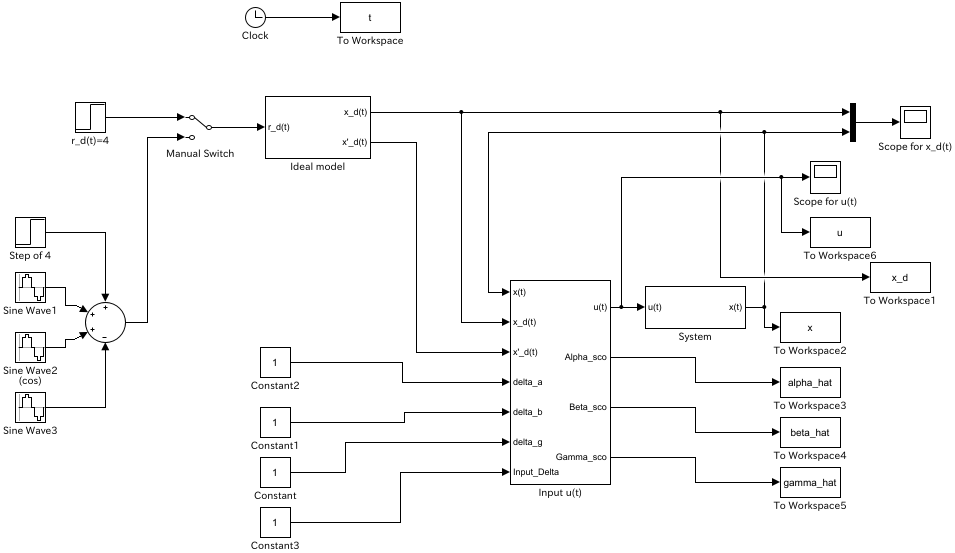
\includegraphics[scale=0.6]{../figure/fig/structured_model.png}
  \caption{構成したモデルの全体図}
  \label{structured_model}
 \end{center}
\end{figure}
%=================================================
\begin{figure}[H]
 \begin{center}
  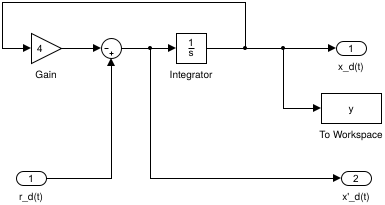
\includegraphics[scale=0.6]{../figure/fig/ideal_model.png}
  \caption{理想モデル}
  \label{ideal_model}
 \end{center}
\end{figure}
%=================================================
\begin{figure}[H]
 \begin{center}
  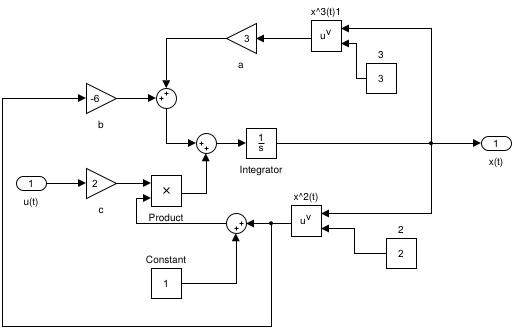
\includegraphics[scale=0.6]{../figure/fig/controlled_model.png}
  \caption{制御対象}
  \label{controlled_model}
 \end{center}
\end{figure}
%=================================================
\begin{figure}[H]
 \begin{center}
  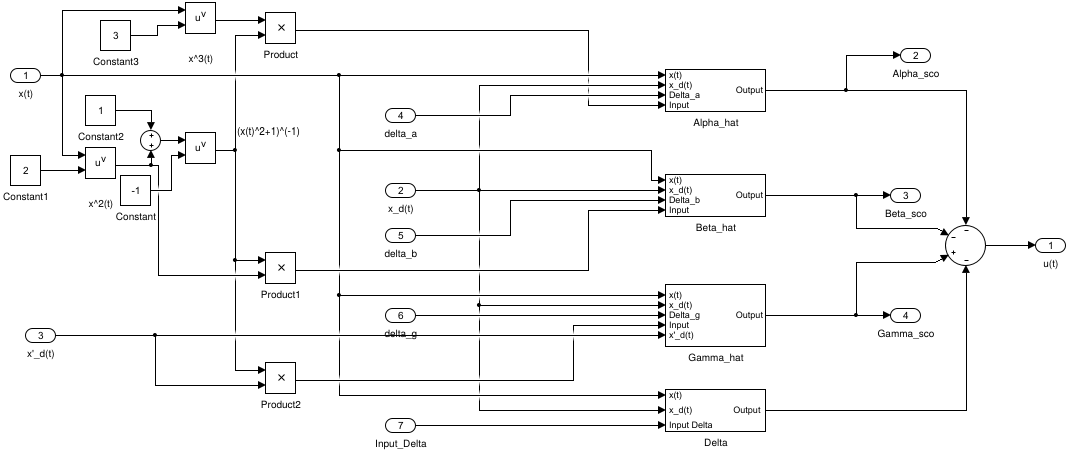
\includegraphics[scale=0.6]{../figure/fig/input.png}
  \caption{入力u(t)}
  \label{controlled_model}
 \end{center}
\end{figure}
%=================================================
\begin{figure}[H]
 \centering
 \subfloat[$\hat{\alpha}$の推定器]{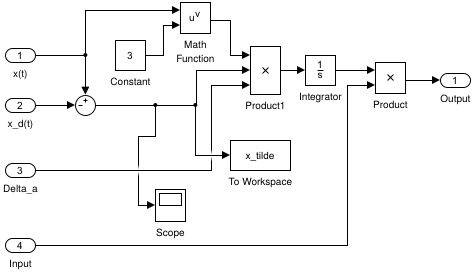
\includegraphics[scale=0.6]{../figure/fig/alpha_hat.png}}
 \hspace{1.5cm}
 \subfloat[$\hat{\beta}$の推定器]{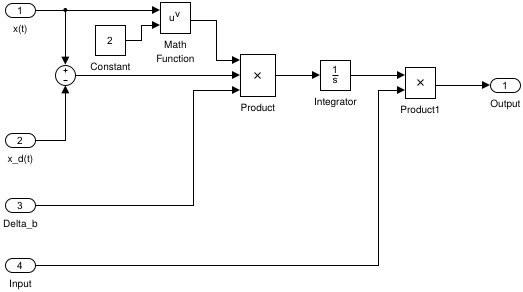
\includegraphics[scale=0.55]{../figure/fig/beta_hat.png}}
\\
 \vspace{0.5cm}
 \subfloat[$\hat{\gamma}$の推定器]{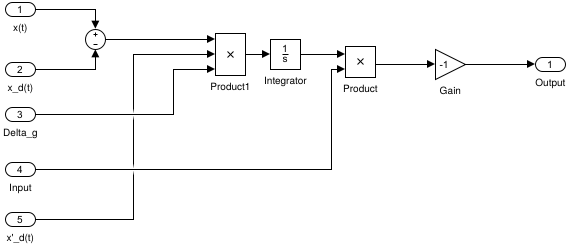
\includegraphics[scale=0.55]{../figure/fig/gamma_hat.png}}
\\
 \caption{各推定器のモデル}
 \label{hats}
\end{figure}
%=================================================
\begin{figure}[H]
 \begin{center}
  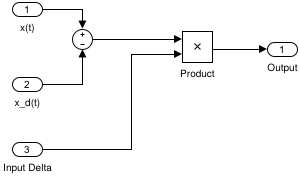
\includegraphics[scale=0.8]{../figure/fig/delta.png}
  \caption{$\delta$に関するサブシステム}
  \label{delta}
 \end{center}
\end{figure}
%=================================================
%=================================================
\subsection{シミュレーション結果}
%=================================================
%\subsubsection{$ r_d(t) = 4 $の場合}
\subsubsection{入力ゲインのみを変化させた場合}
%=================================================
まず,入力ゲインのみを変化させる.適応ゲインは$ \delta_{\alpha} = \delta_{\beta} = \delta_{\gamma} = 1 $とした.式({\ref{ideal}})について$ r_d(t) = 4 $の場合のシミュレーション結果を{\bf Fig.}{\ref{x1}}〜{\ref{hats1}}に示す.
%=================================================
\begin{figure}[H]
 \begin{center}
  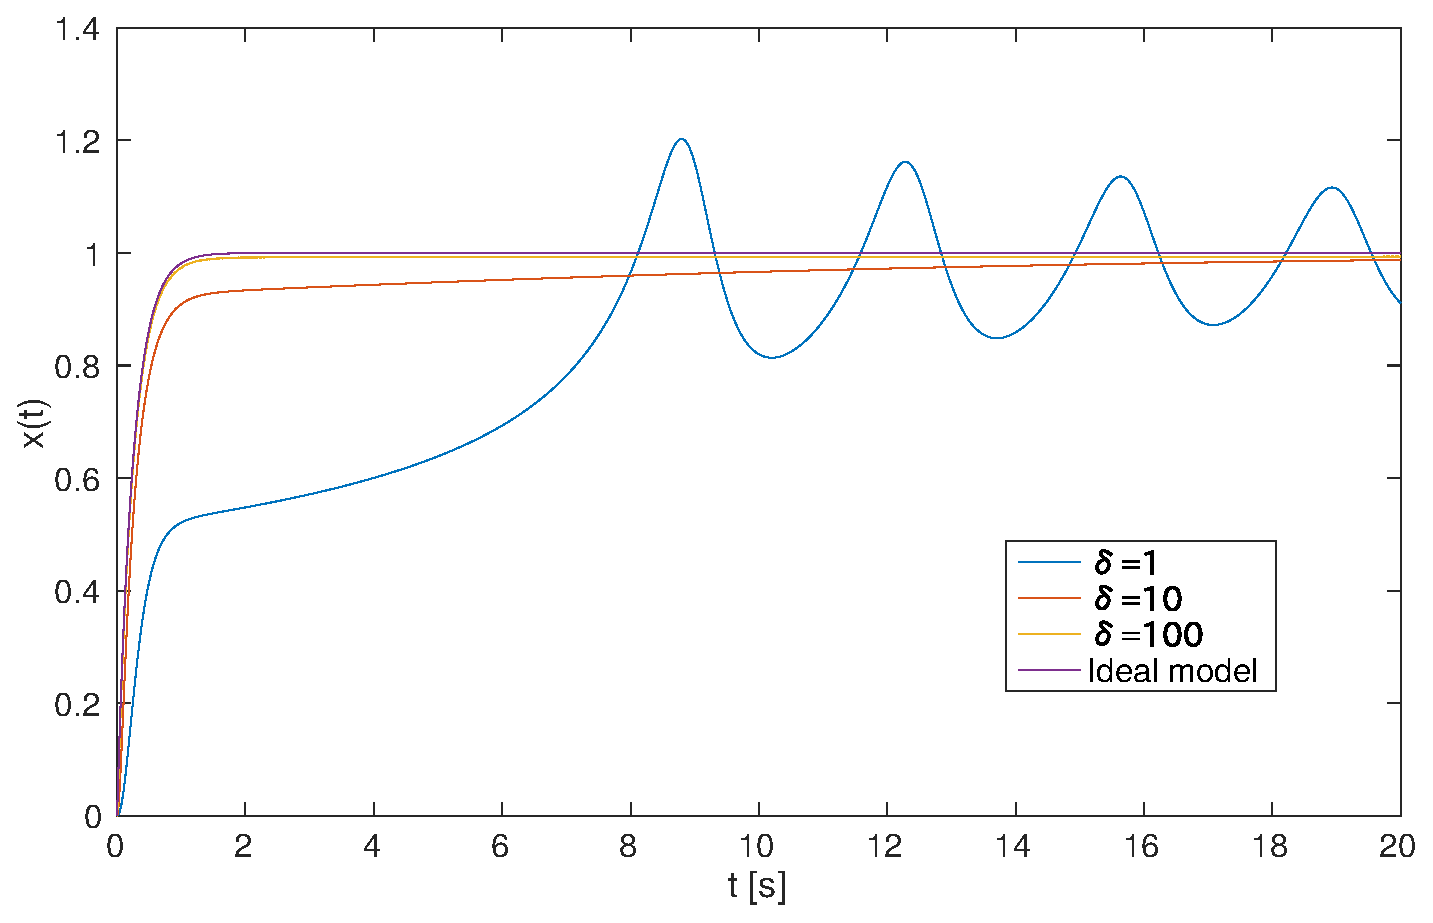
\includegraphics[scale=0.485]{../figure/eps/input/1/x.eps}
  \caption{$ r_d = 4 $のときの理想軌道と出力$ x(t) $の比較$(\delta = 1, ~ 10, ~ 100 )$}
  \label{x1}
 \end{center}
\end{figure}
%=================================================
\begin{figure}[H]
 \begin{center}
  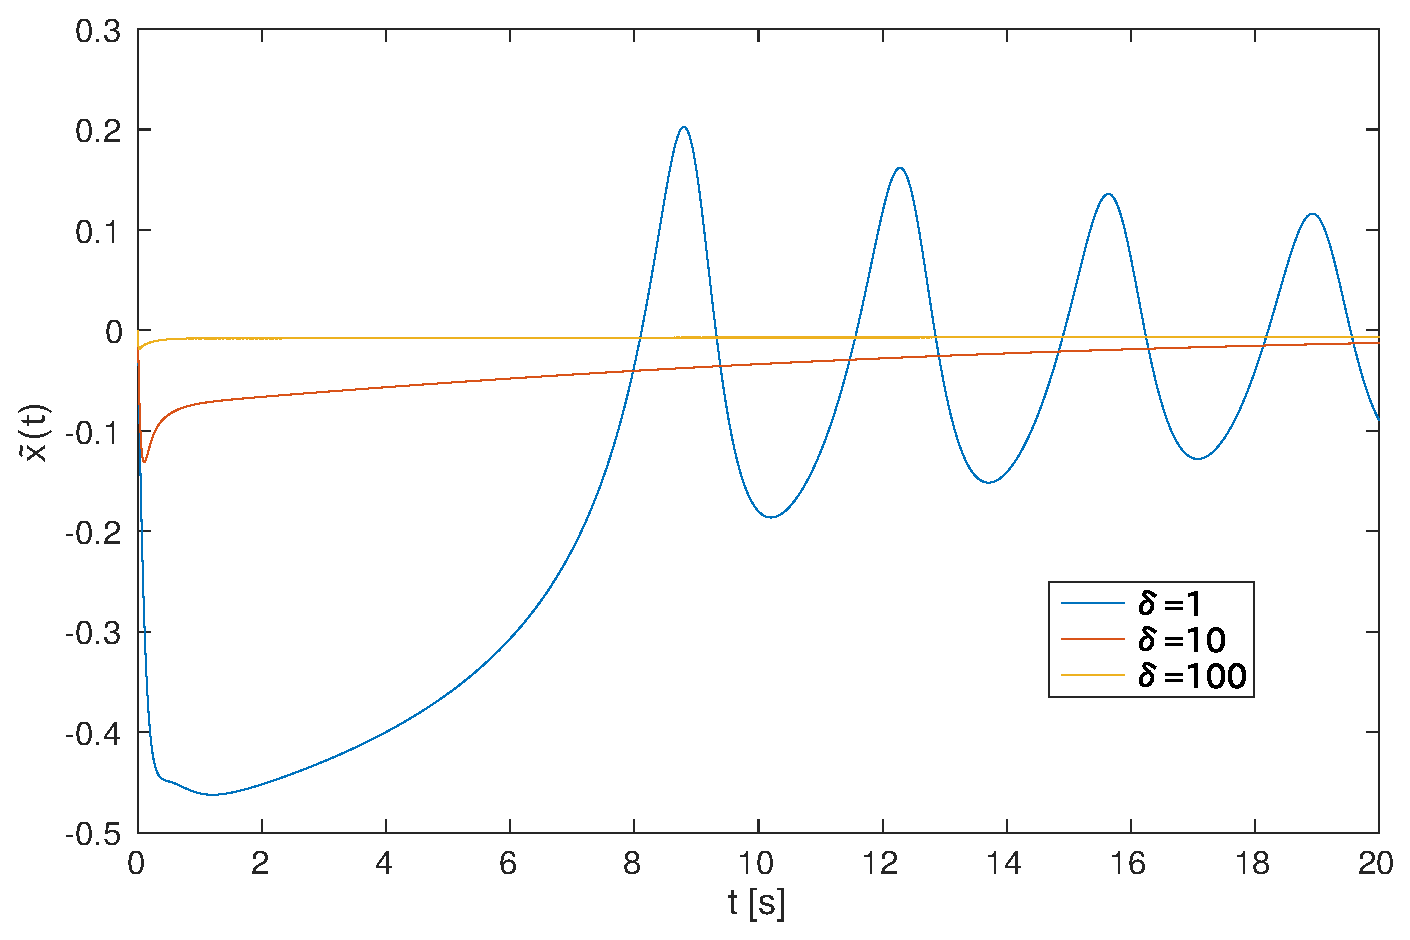
\includegraphics[scale=0.5]{../figure/eps/input/1/tilde_x.eps}
  \caption{$ r_d = 4 $のときの追従誤差$ \tilde{x}(t) $の変化$(\delta = 1, ~ 10, ~ 100 )$}
  \label{tilde_x1}
 \end{center}
\end{figure}
%=================================================
\begin{figure}[H]
 \begin{center}
  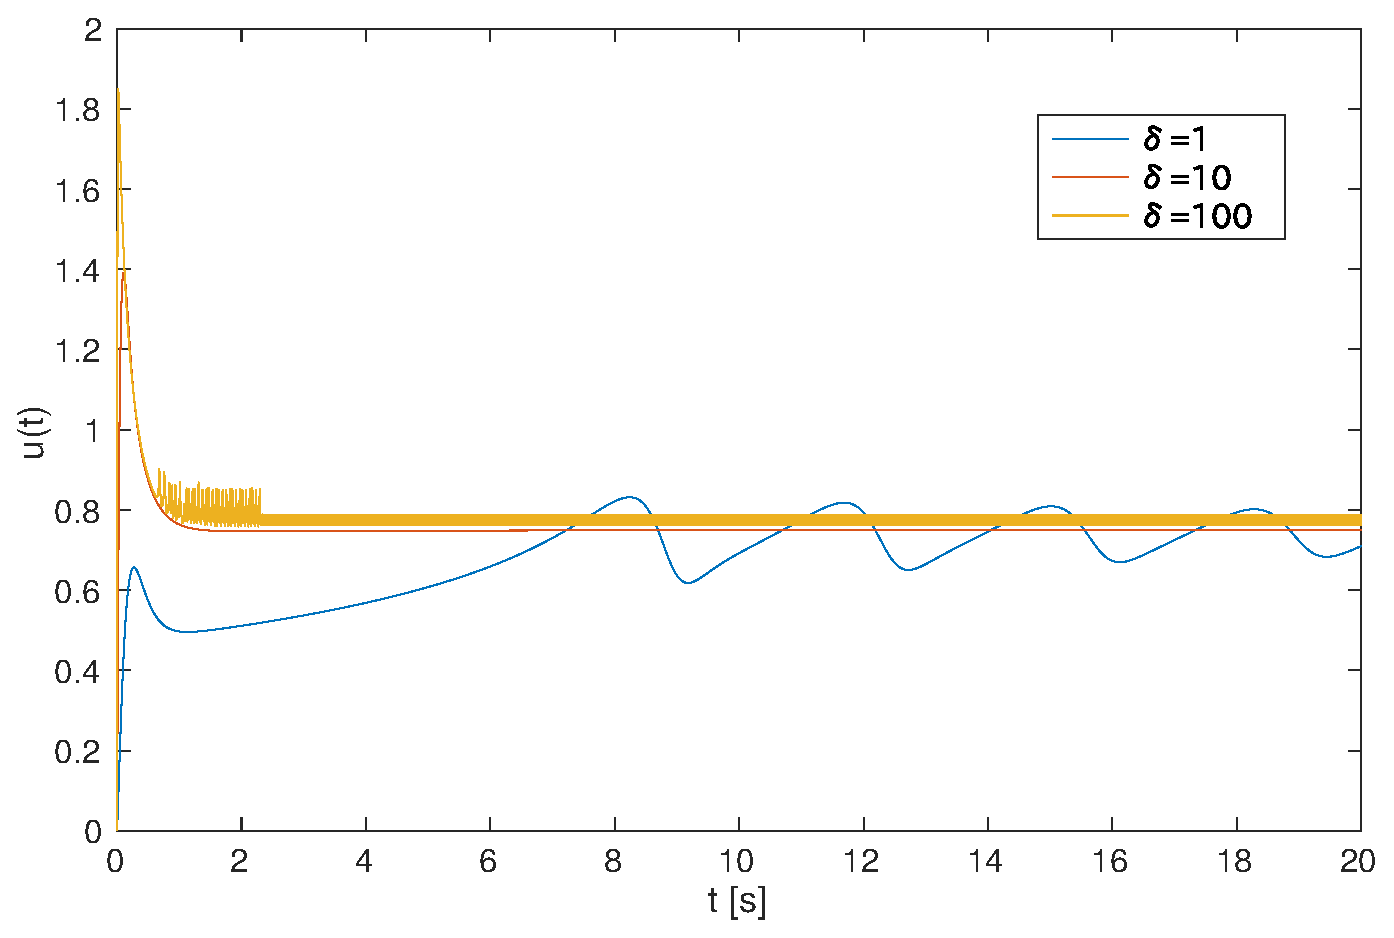
\includegraphics[scale=0.5]{../figure/eps/input/1/u.eps}
  \caption{$ r_d = 4 $のときの入力$ u(t) $の変化$(\delta = 1, ~ 10, ~ 100 )$}
  \label{u1}
 \end{center}
\end{figure}
%=================================================
\begin{figure}[H]
 \centering
 \subfloat[$ \hat{\alpha} $の出力]{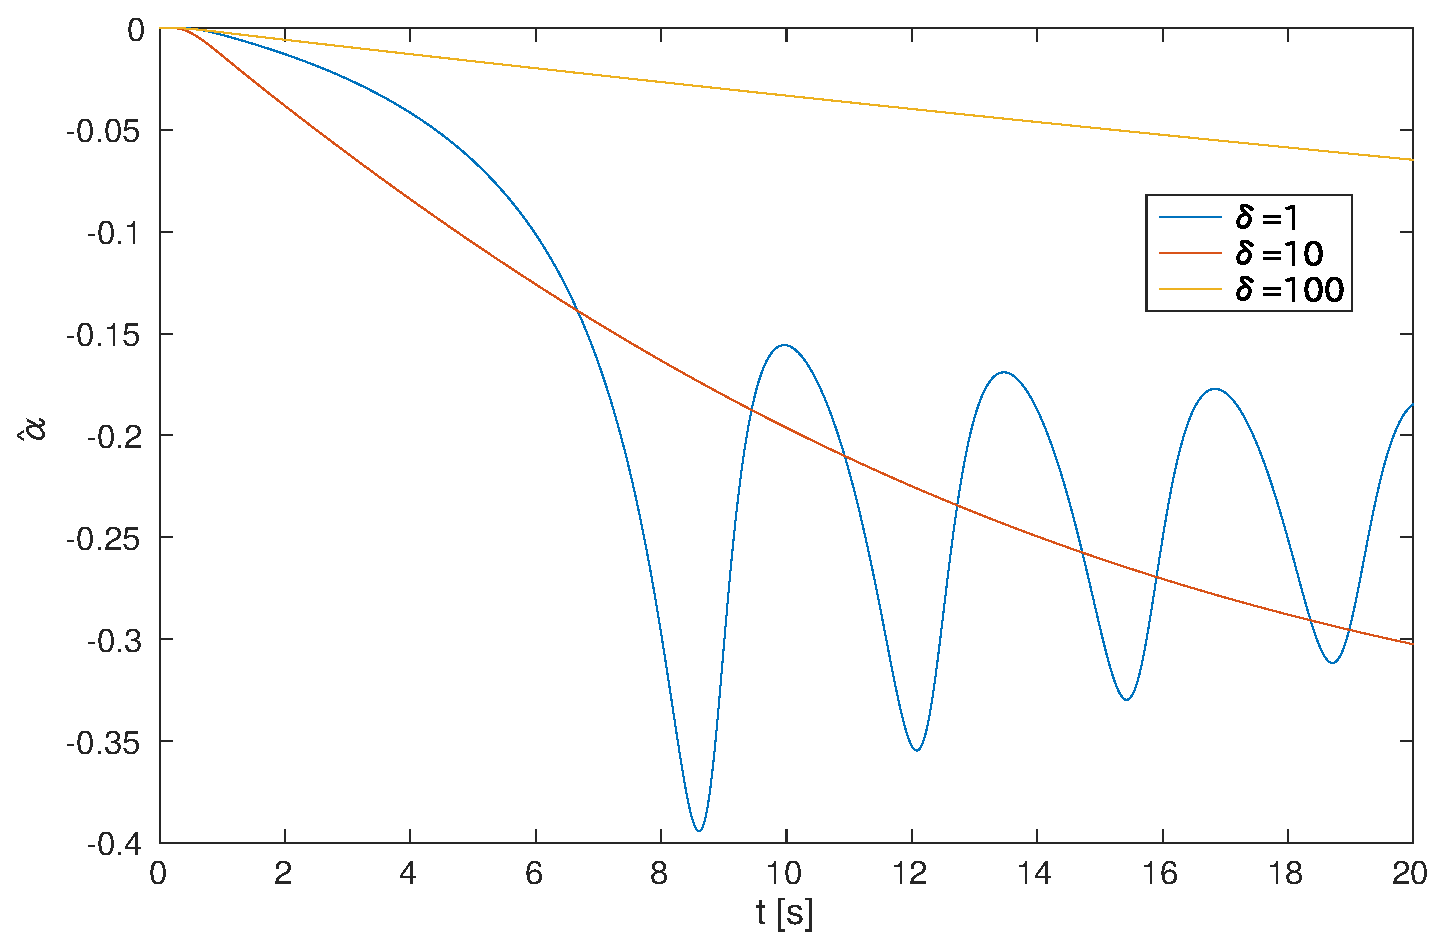
\includegraphics[scale=0.35]{../figure/eps/input/1/alpha_hat.eps}}
 \hspace{0.1cm}
 \subfloat[$ \hat{\beta} $の出力]{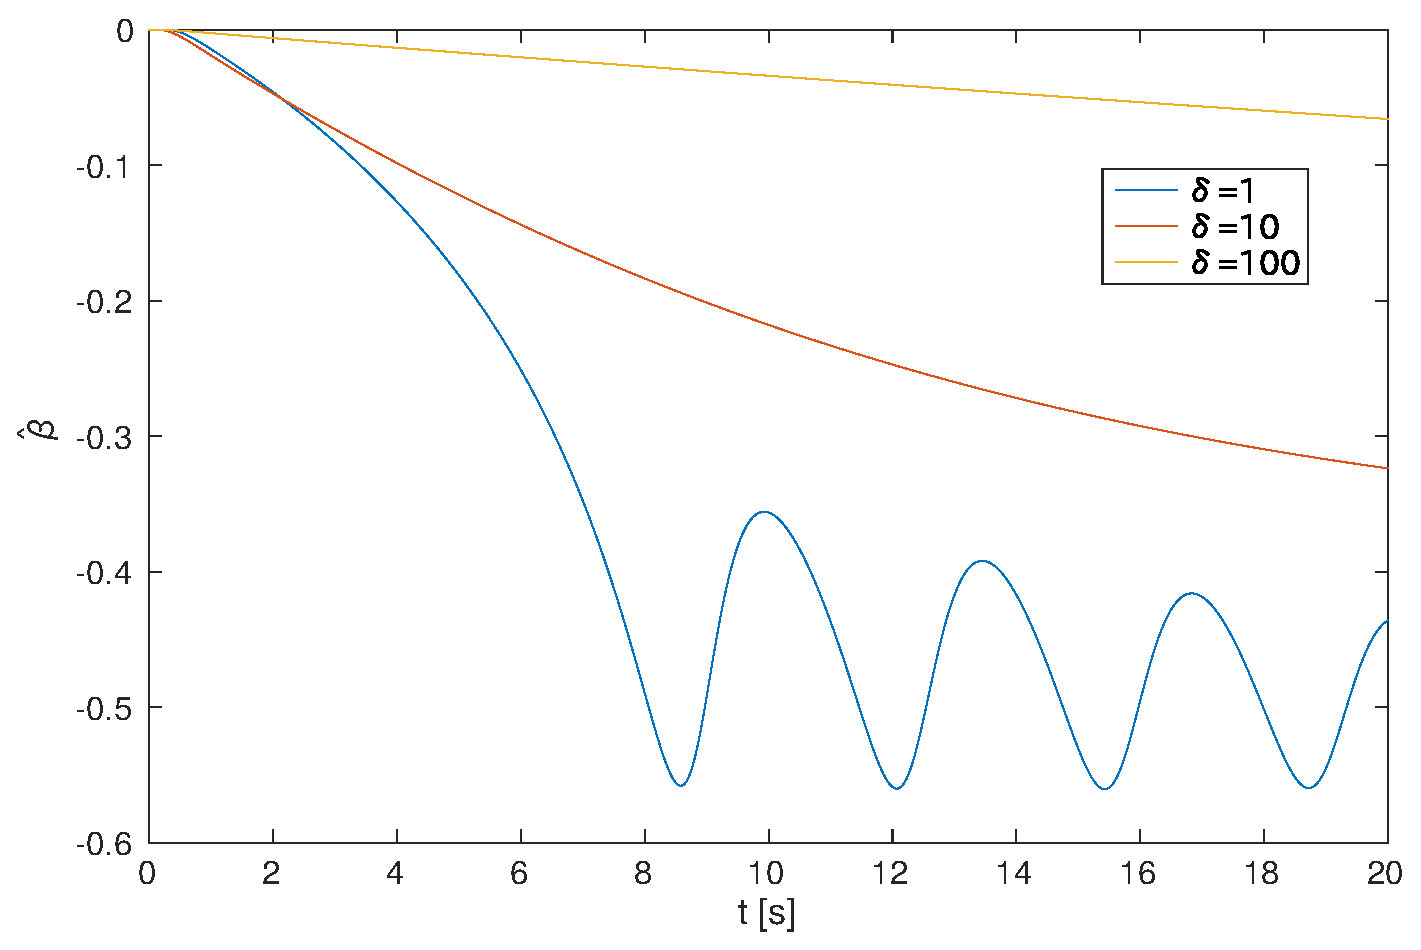
\includegraphics[scale=0.35]{../figure/eps/input/1/beta_hat.eps}}
\\
 \vspace{0.5cm}
 \subfloat[$ \hat{\gamma} $の出力]{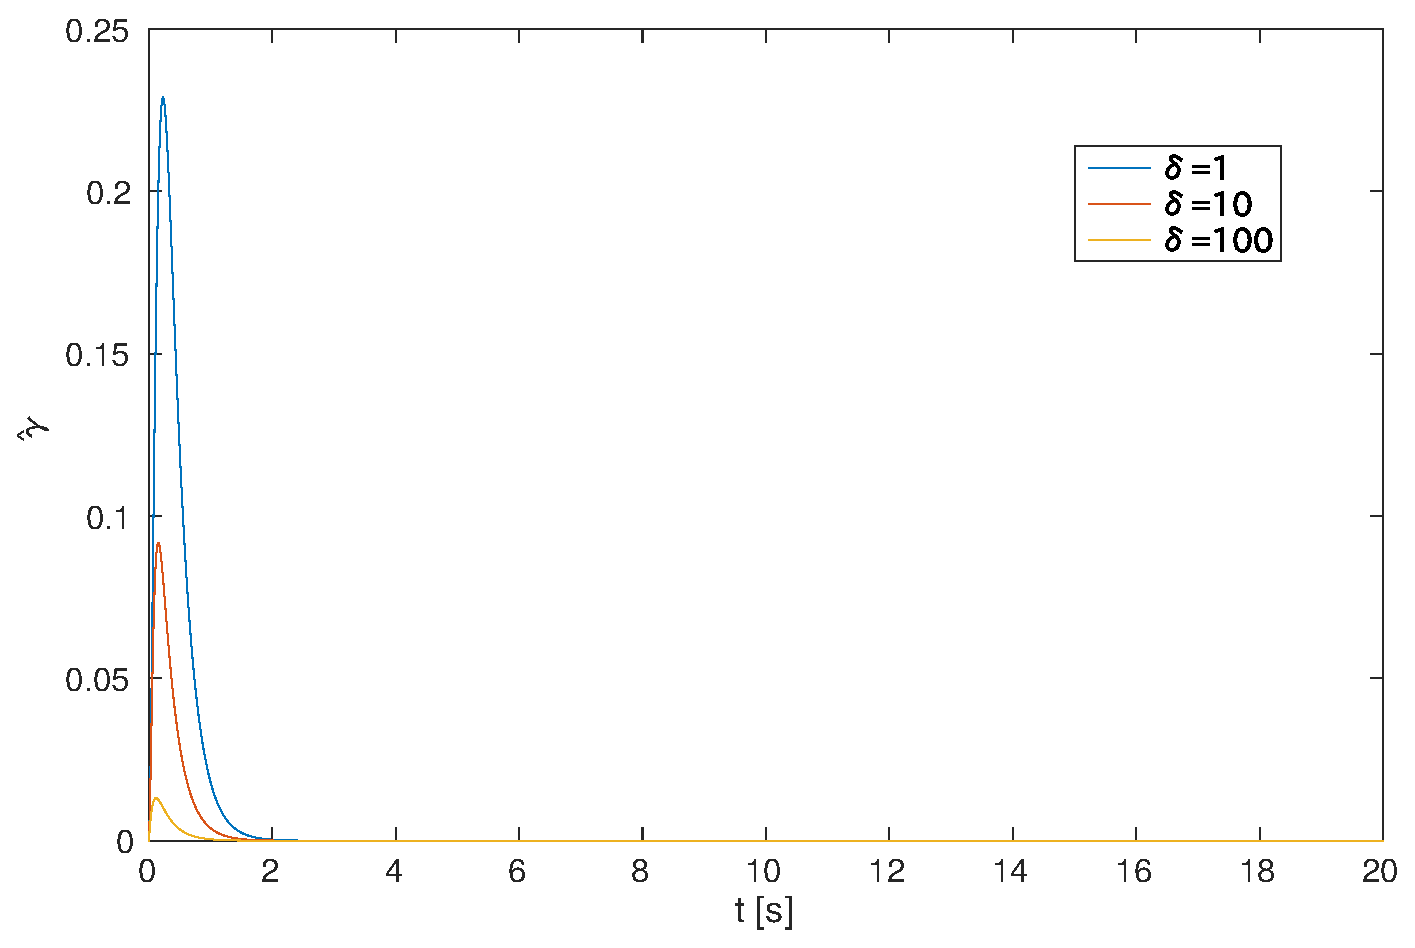
\includegraphics[scale=0.38]{../figure/eps/input/1/gamma.eps}}
 \caption{$ r_d = 4 $のときの各推定器の出力$ (\delta = 1, ~ 10, ~ 100) $}
 \label{hats1}
\end{figure}
%=================================================
次に,$ r_d = 4 + 0.5{\rm sin}0.5t + {\rm cos}3t -2{\rm sin}5t $の場合のシミュレーション結果を{\bf Fig.}{\ref{x2}}〜{\ref{hats2}}に示す.このときの適応ゲインは先程の$ r_d = 4 $のときと同様である.
%=================================================
\begin{figure}[H]
 \begin{center}
  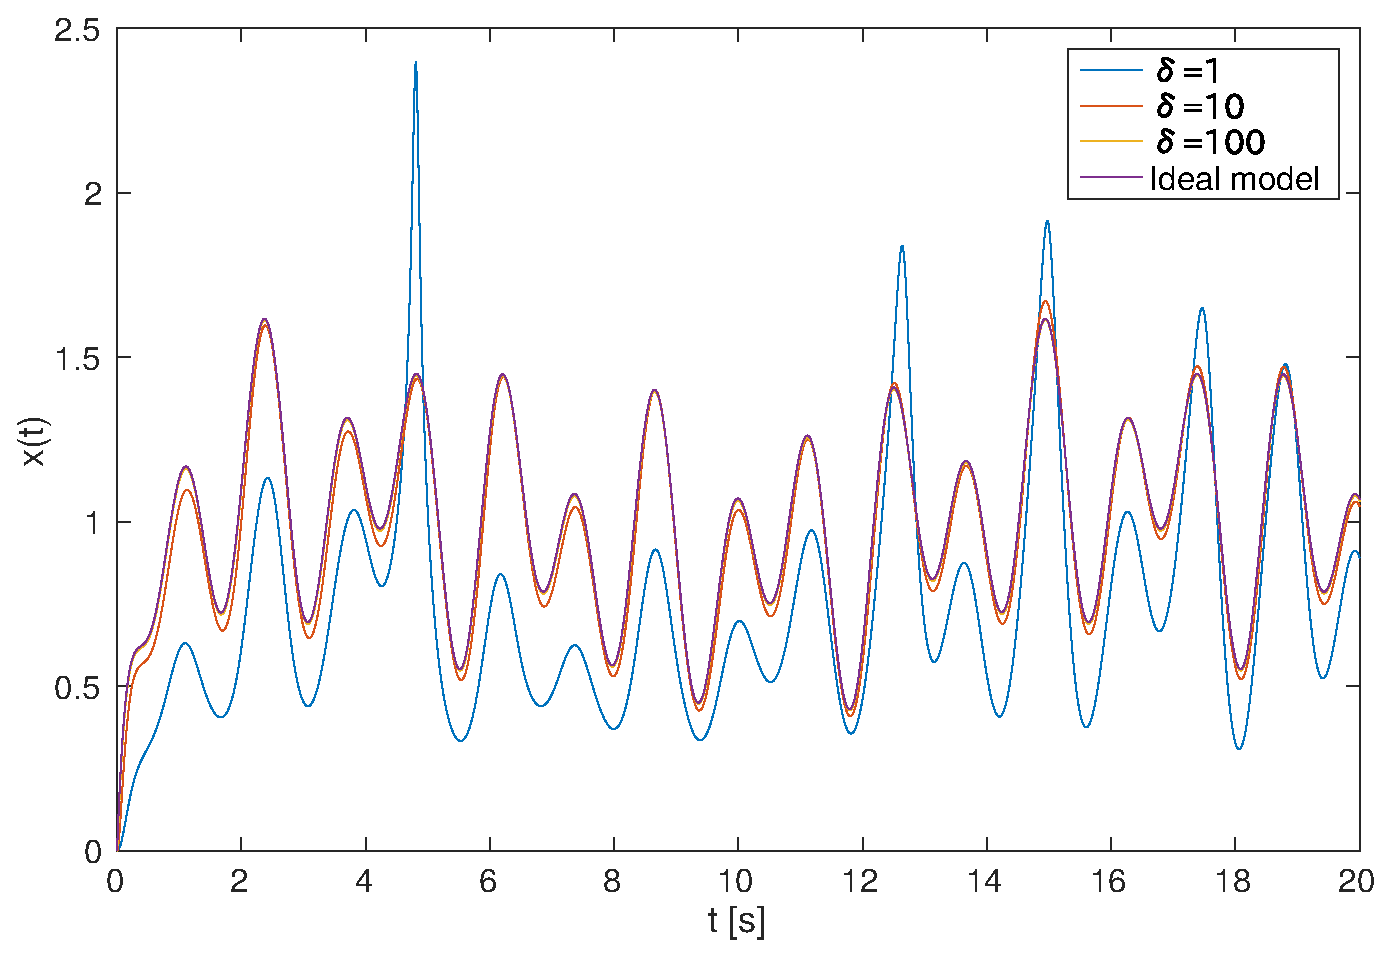
\includegraphics[scale=0.485]{../figure/eps/input/2/x.eps}
  \caption{$ r_d = 4 + 0.5{\rm sin}0.5t + {\rm cos}3t -2{\rm sin}5t $のときの理想軌道と出力$ x(t) $の比較$(\delta = 1, ~ 10, ~ 100 )$}
  \label{x2}
 \end{center}
\end{figure}
%=================================================
\begin{figure}[H]
 \begin{center}
  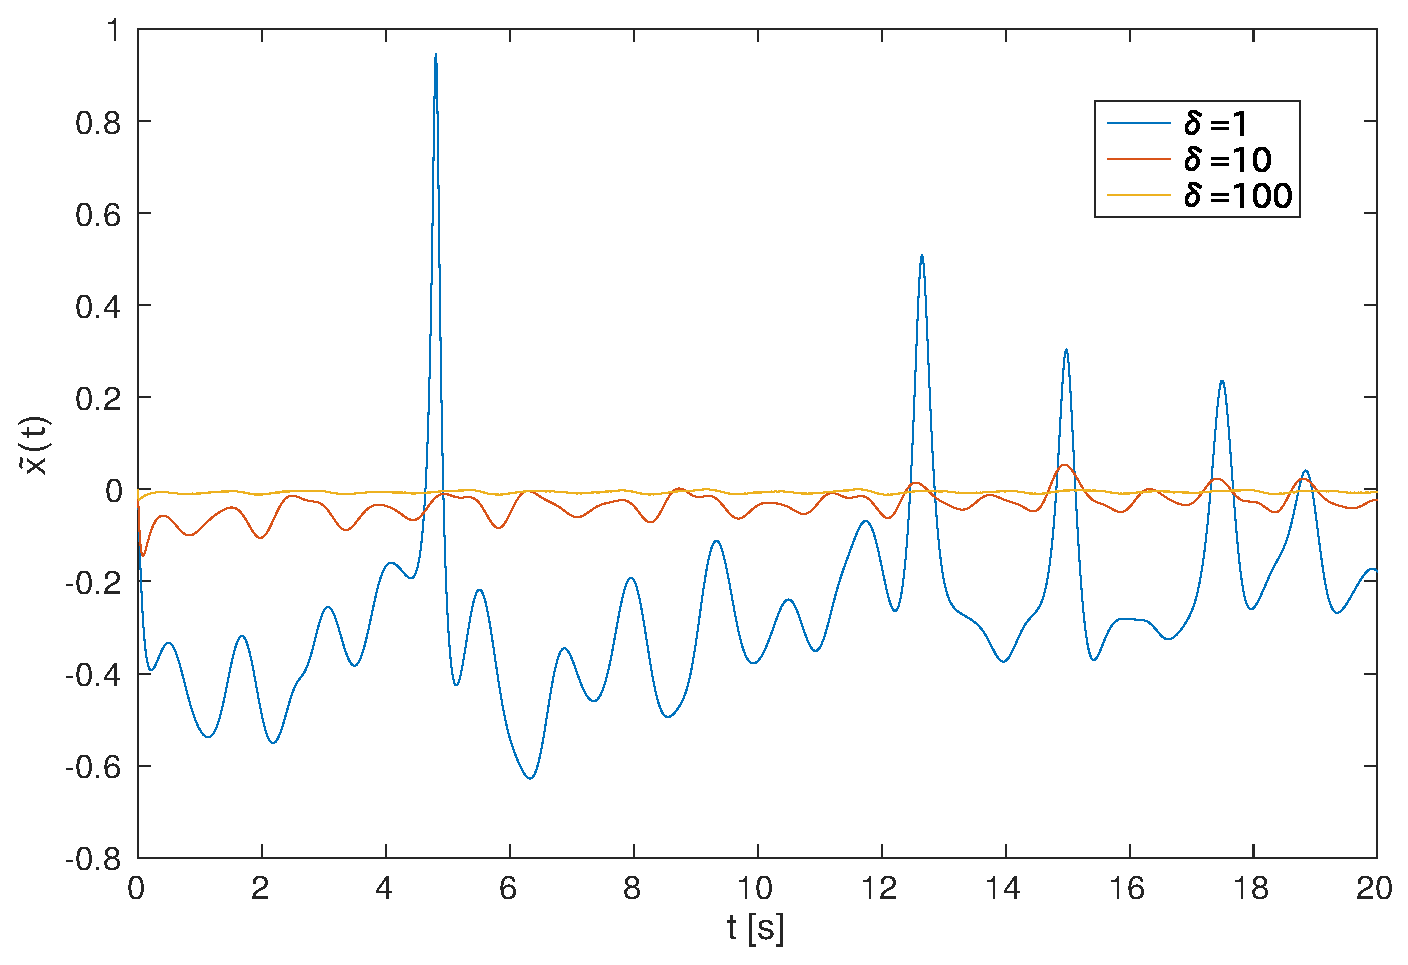
\includegraphics[scale=0.5]{../figure/eps/input/2/tilde_x.eps}
  \caption{$ r_d = 4 + 0.5{\rm sin}0.5t + {\rm cos}3t -2{\rm sin}5t $のときの追従誤差$ \tilde{x}(t) $の変化$(\delta = 1, ~ 10, ~ 100 )$}
  \label{tilde_x2}
 \end{center}
\end{figure}
%=================================================
\begin{figure}[H]
 \begin{center}
  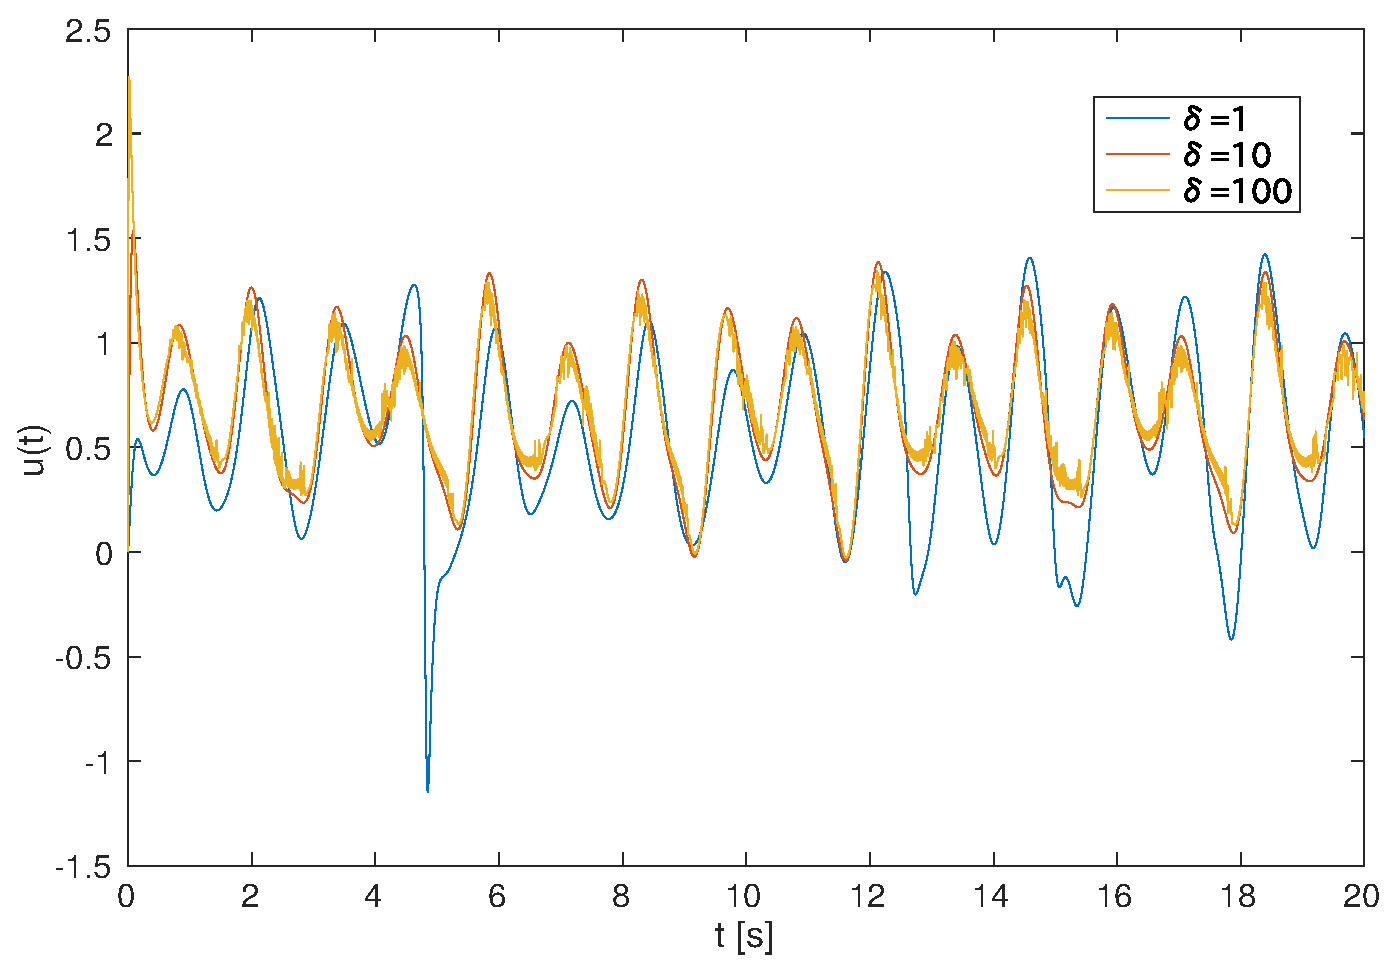
\includegraphics[scale=0.5]{../figure/eps/input/2/u.eps}
  \caption{$ r_d = 4 + 0.5{\rm sin}0.5t + {\rm cos}3t -2{\rm sin}5t $のときの入力$ u(t) $の変化$(\delta = 1, ~ 10, ~ 100 )$}
  \label{u2}
 \end{center}
\end{figure}
%=================================================
\begin{figure}[H]
 \centering
 \subfloat[$ \hat{\alpha} $の出力]{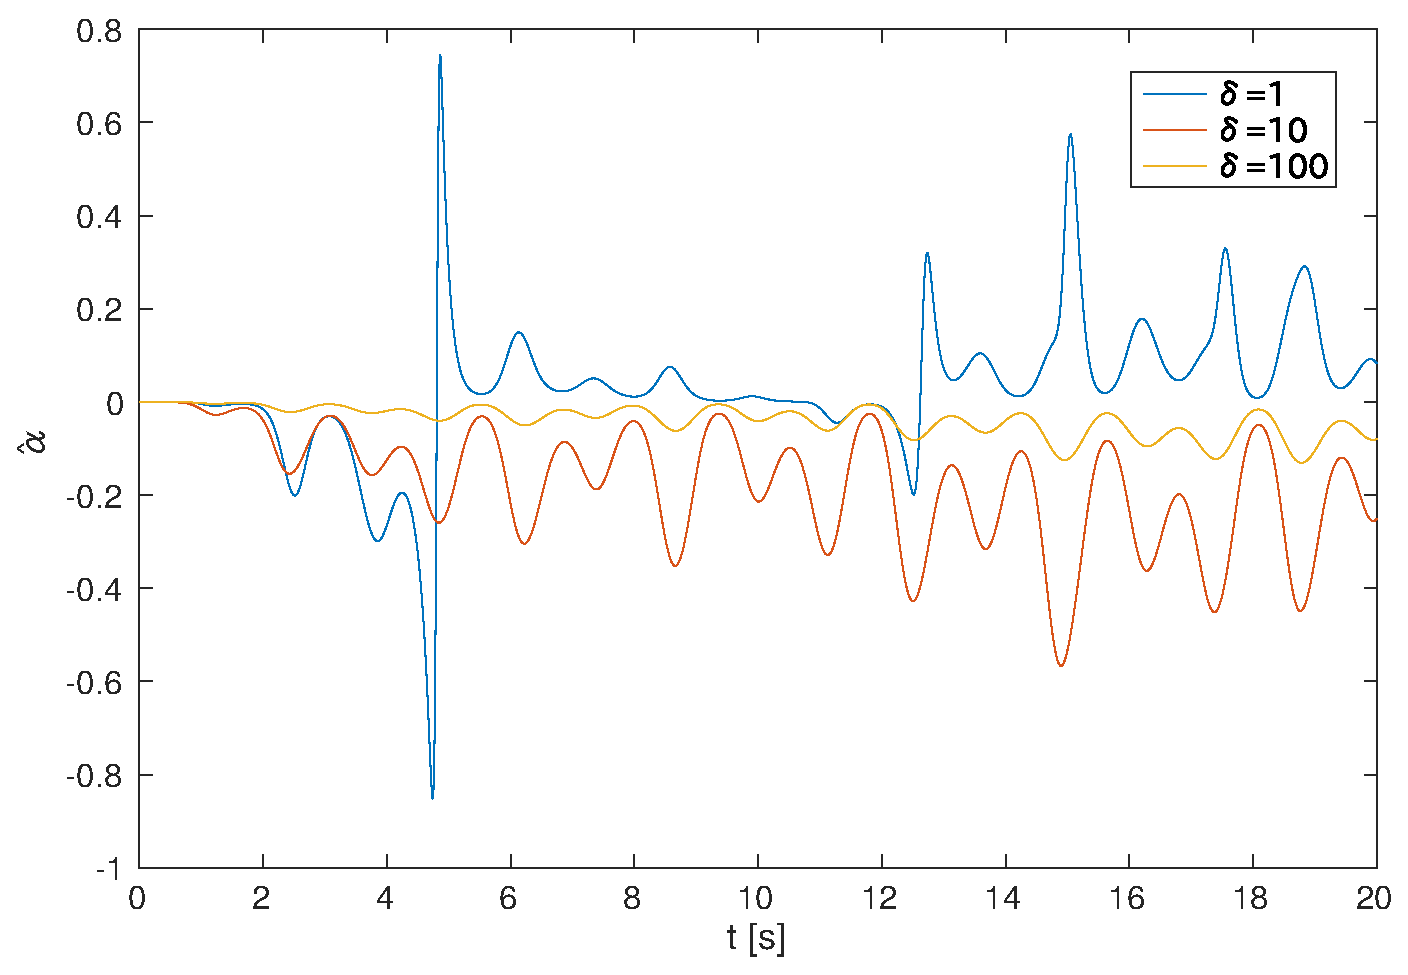
\includegraphics[scale=0.35]{../figure/eps/input/2/alpha_hat.eps}}
 \hspace{0.1cm}
 \subfloat[$ \hat{\beta} $の出力]{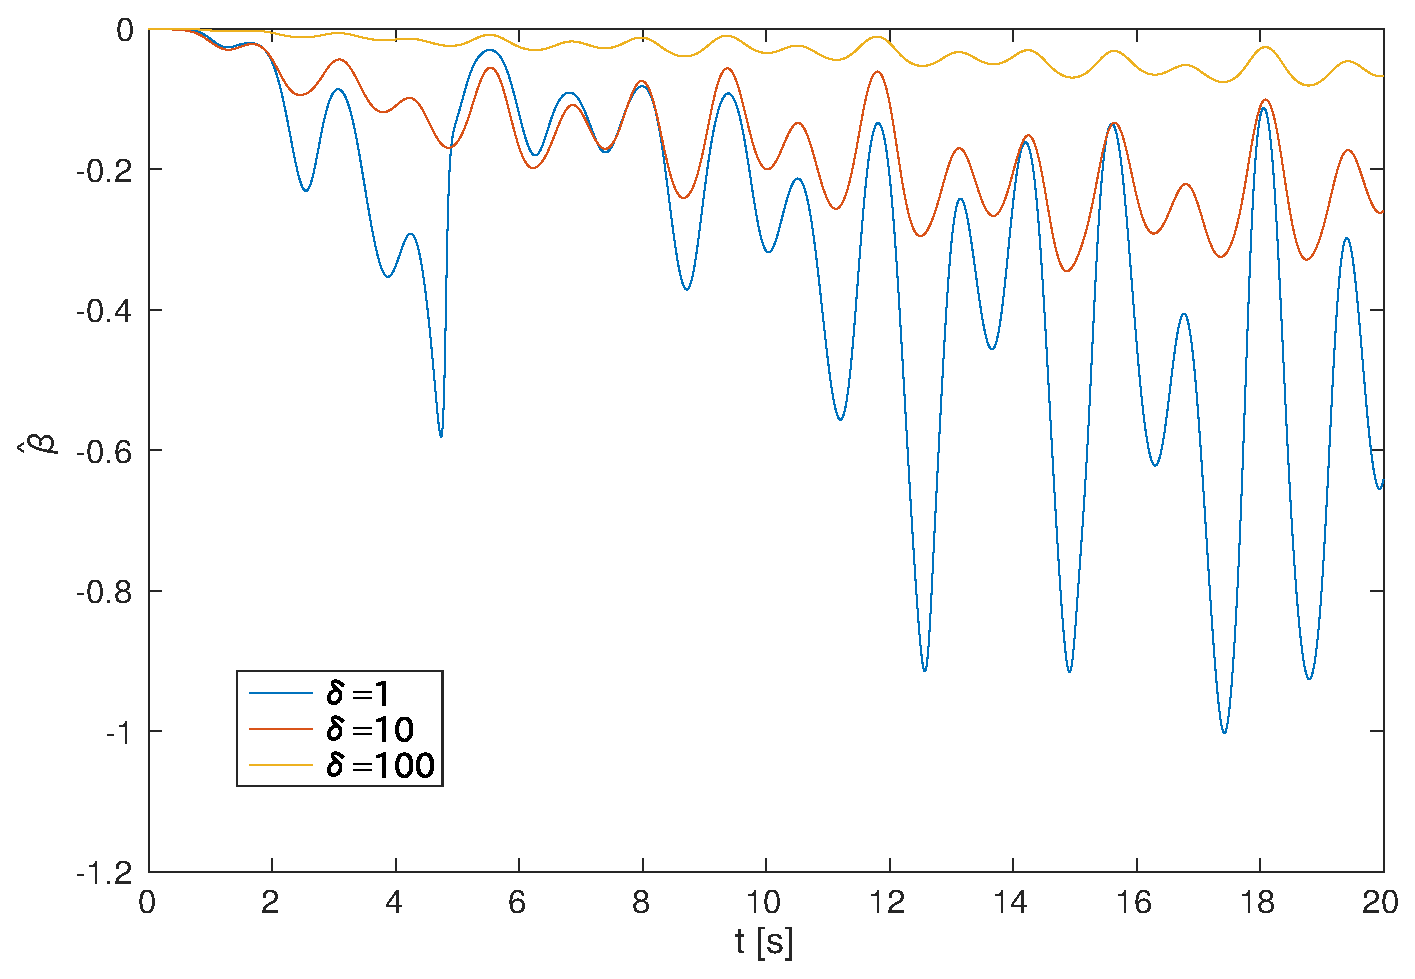
\includegraphics[scale=0.35]{../figure/eps/input/2/beta_hat.eps}}
\\
 \vspace{0.5cm}
 \subfloat[$ \hat{\gamma} $の出力]{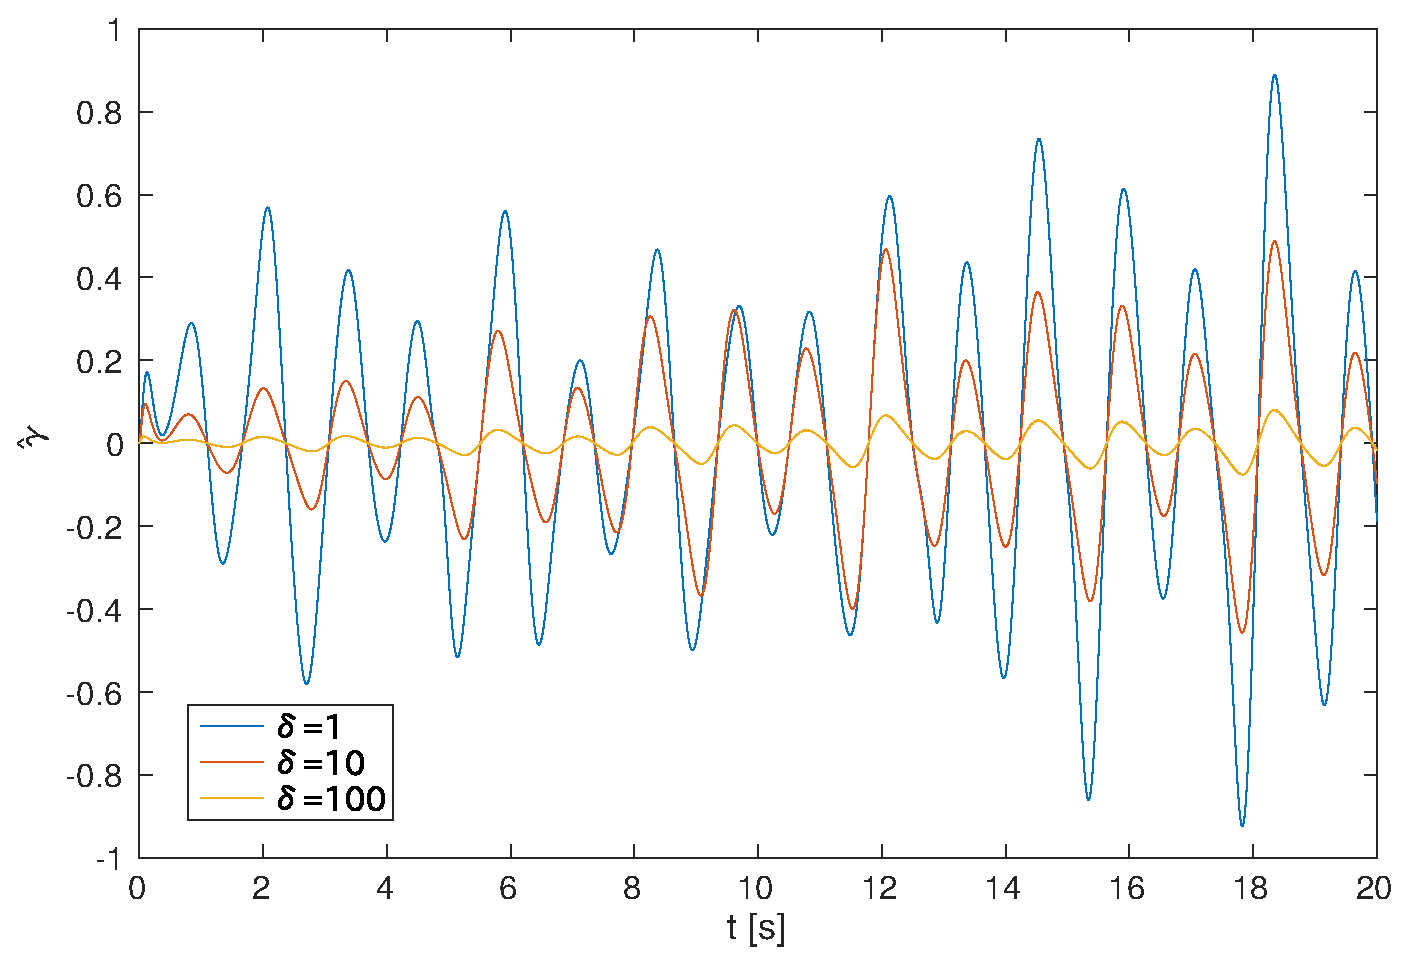
\includegraphics[scale=0.38]{../figure/eps/input/2/gamma_hat.eps}}
 \caption{$ r_d = 4 + 0.5{\rm sin}0.5t + {\rm cos}3t -2{\rm sin}5t $のときの各推定器の出力$( \delta = 1, ~ 10, ~ 100 )$}
 \label{hats2}
\end{figure}
%=================================================
%=================================================
\subsubsection{適応ゲインのみを変化させた場合}
%=================================================
前小々節の結果より,入力ゲイン$ \delta = 100 $としたときが最も理想軌道に近く,追従誤差も0に近いことが分かる.したがってここでは,入力ゲインを$ \delta = 100 $とし,適応ゲインの変化による応答の違いを見る.ここで,設計パラメータの設定方法として次の関係を用いる.
\begin{equation}
 \delta_{\beta} = \delta_{\alpha} , ~~ \delta_{\gamma} = \delta_{\alpha} ^{\frac{3}{2}}
\end{equation}
このように,一つの設計パラメータを用い,それを大きく設定することでより良い制御性能が得られることが知られている{\cite{1}}.本シミュレーションでは,$ \delta_{\alpha} = 100, ~ 1000, ~ 10000 $の三つの場合で応答の様子を調べる.それぞれの対応関係を式で表すと次のようになる.
\begin{eqnarray}
 & \delta_{\alpha} = 100 のとき, & \delta_{\beta} = 100, ~~ \delta_{\gamma} = 1000\\
 & \delta_{\alpha} = 1000 のとき, & \delta_{\beta} = 1000, ~~ \delta_{\gamma} = 31622.7 \dots \simeq 31623 \\
 & \delta_{\alpha} = 10000 のとき, & \delta_{\beta} = 10000, ~~ \delta_{\gamma} = 1000000
\end{eqnarray}

まず,$ r_d = 4 $の場合についてシミュレーションを行なった結果を{\bf Fig.}{\ref{xa1}}〜{\bf Fig.}{\ref{hatsa1}}に示す.
%=================================================
\begin{figure}[H]
 \begin{center}
  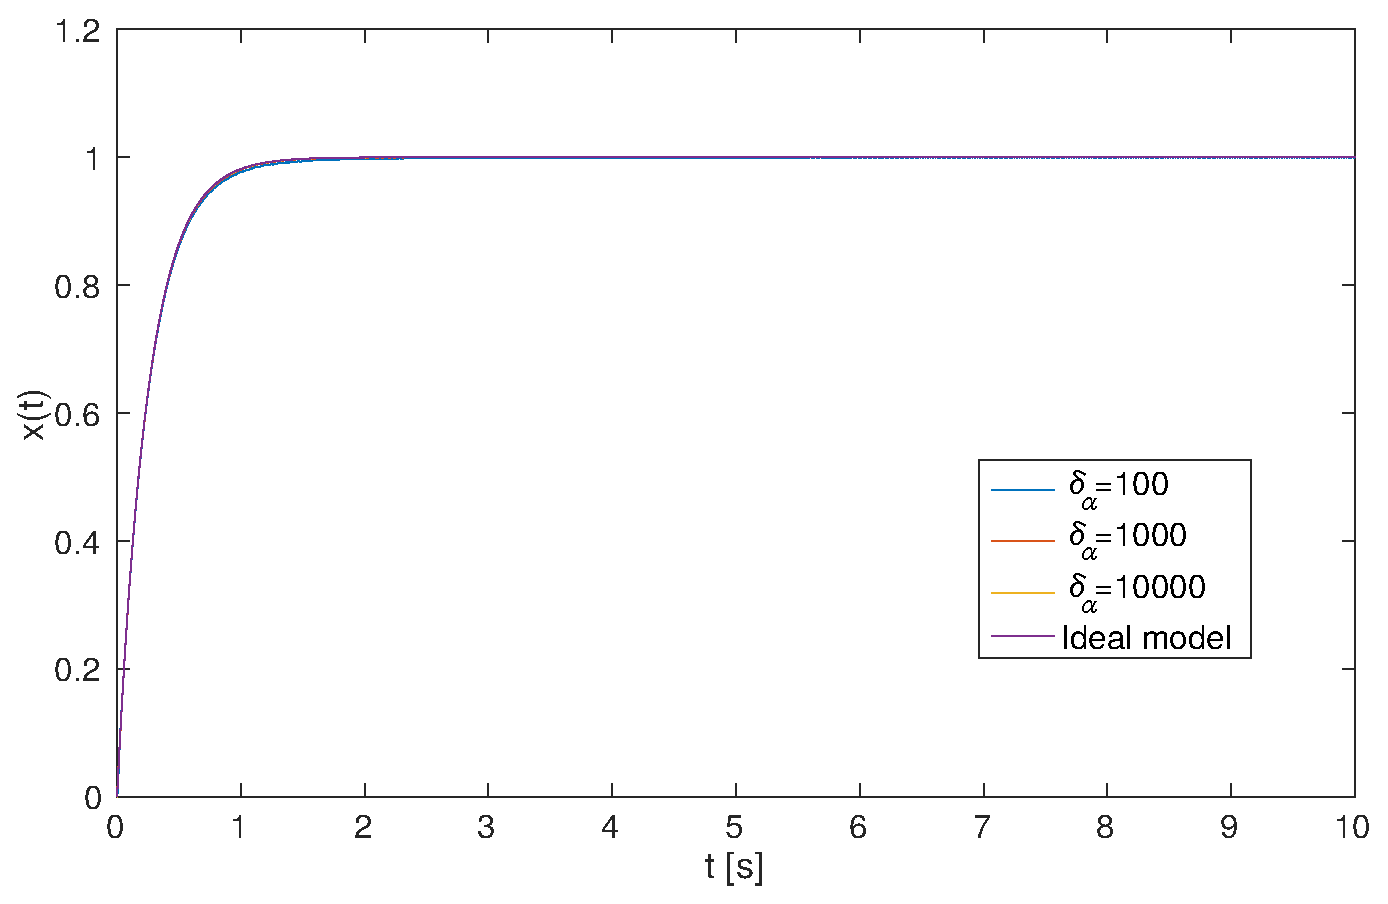
\includegraphics[scale=0.485]{../figure/eps/estimate/1/x.eps}
  \caption{$ r_d = 4 $のときの理想軌道と$ x(t) $の比較$(\delta_{\alpha} = 100, ~ 1000, ~ 10000 )$}
  \label{xa1}
 \end{center}
\end{figure}
%=================================================
\begin{figure}[H]
 \begin{center}
  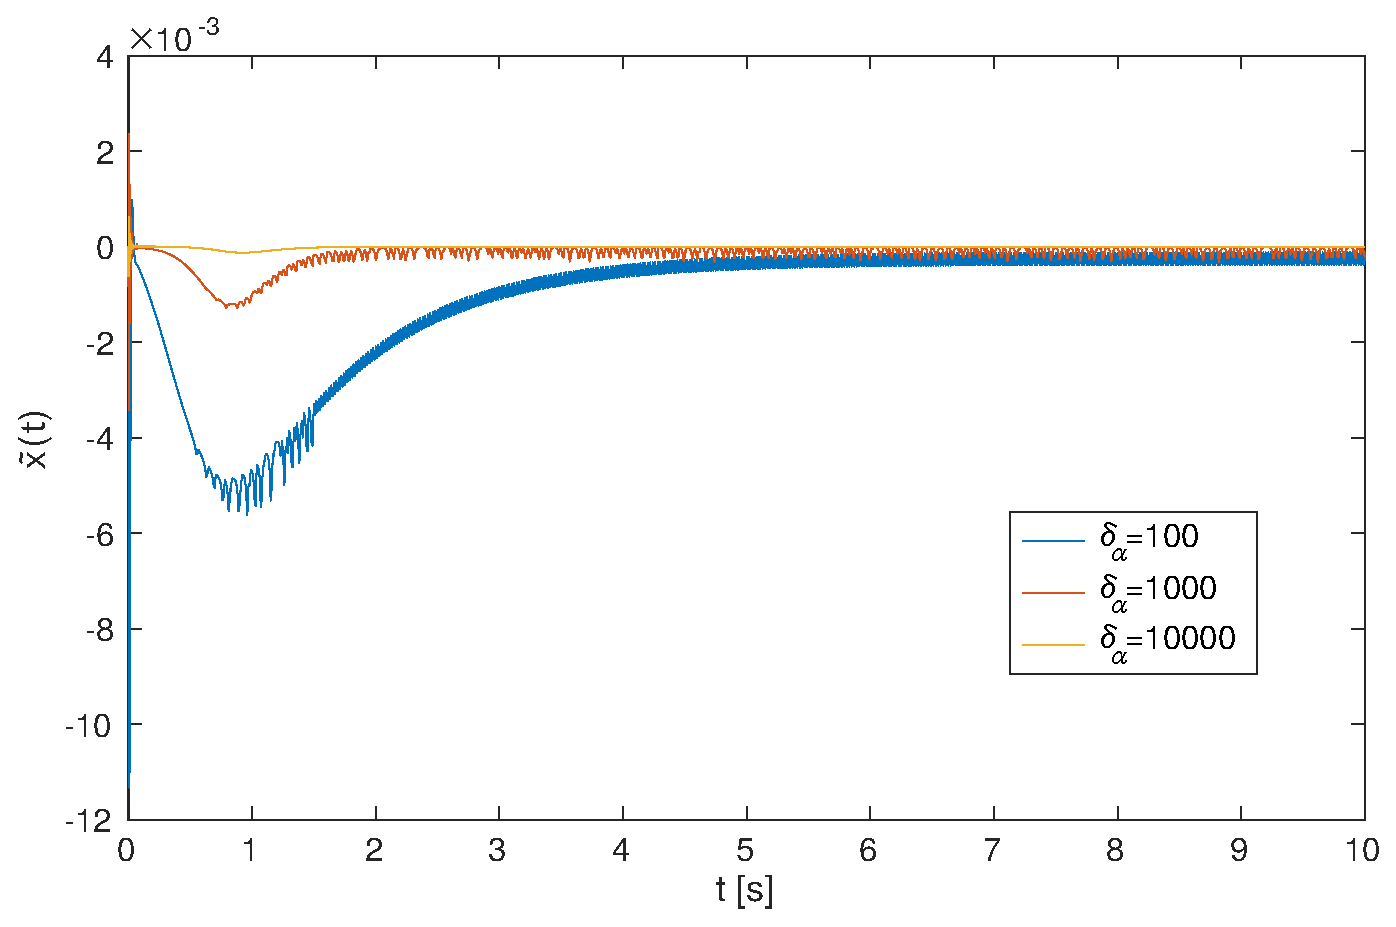
\includegraphics[scale=0.5]{../figure/eps/estimate/1/tilde_x.eps}
  \caption{$ r_d = 4 $のときの追従誤差$ \tilde{x}(t) $の変化$(\delta_{\alpha} = 100, ~ 1000, ~ 10000 )$}
  \label{tilde_xa1}
 \end{center}
\end{figure}
%=================================================
\begin{figure}[H]
 \begin{center}
  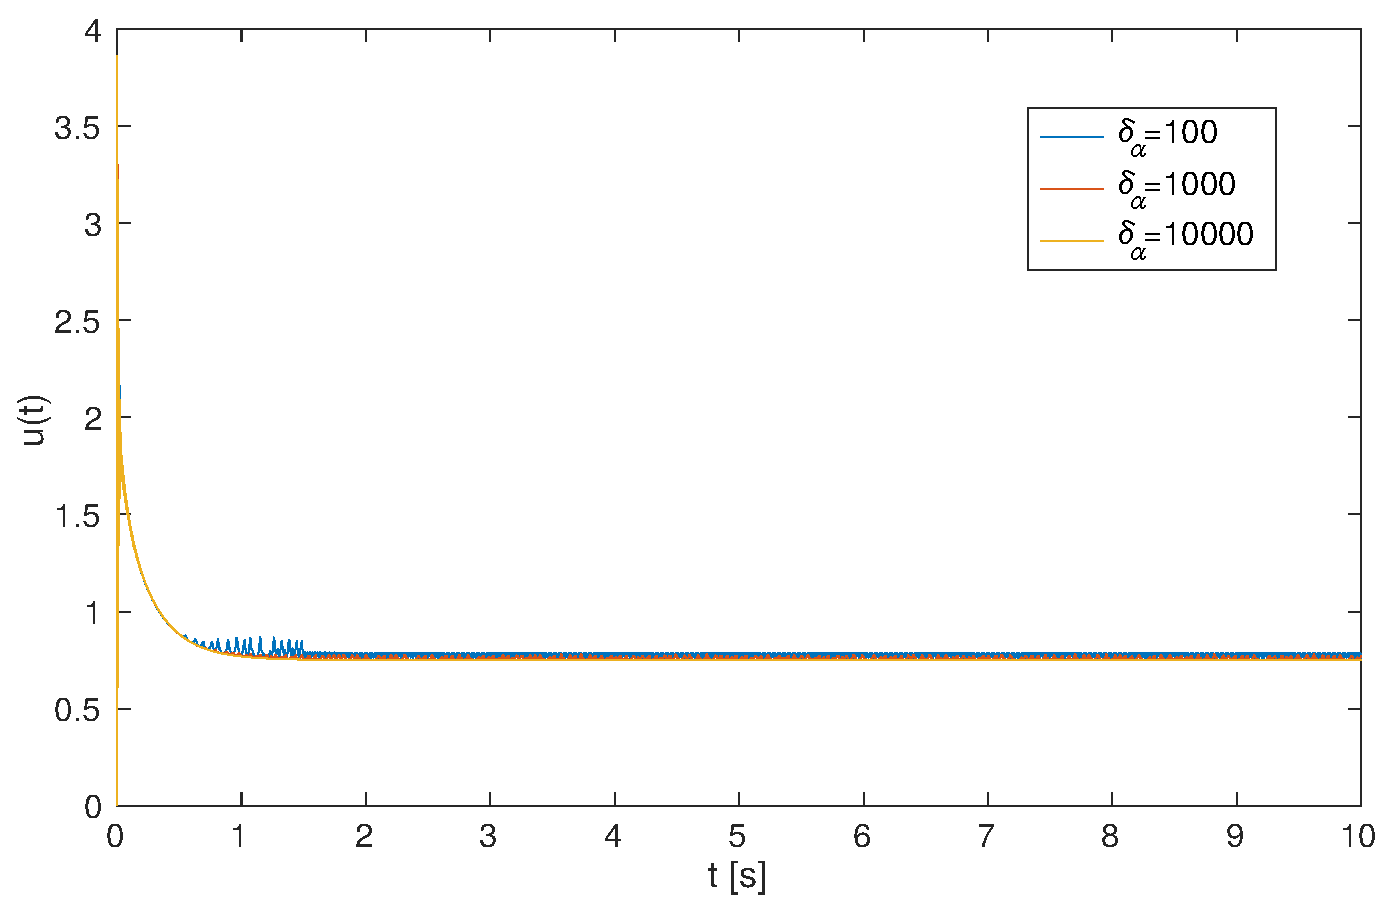
\includegraphics[scale=0.5]{../figure/eps/estimate/1/u.eps}
  \caption{$ r_d = 4 $のときの入力$ u(t) $の変化$(\delta_{\alpha} = 100, ~ 1000, ~ 10000 )$}
  \label{ua1}
 \end{center}
\end{figure}
%=================================================
\begin{figure}[H]
 \centering
 \subfloat[$ \hat{\alpha} $の出力]{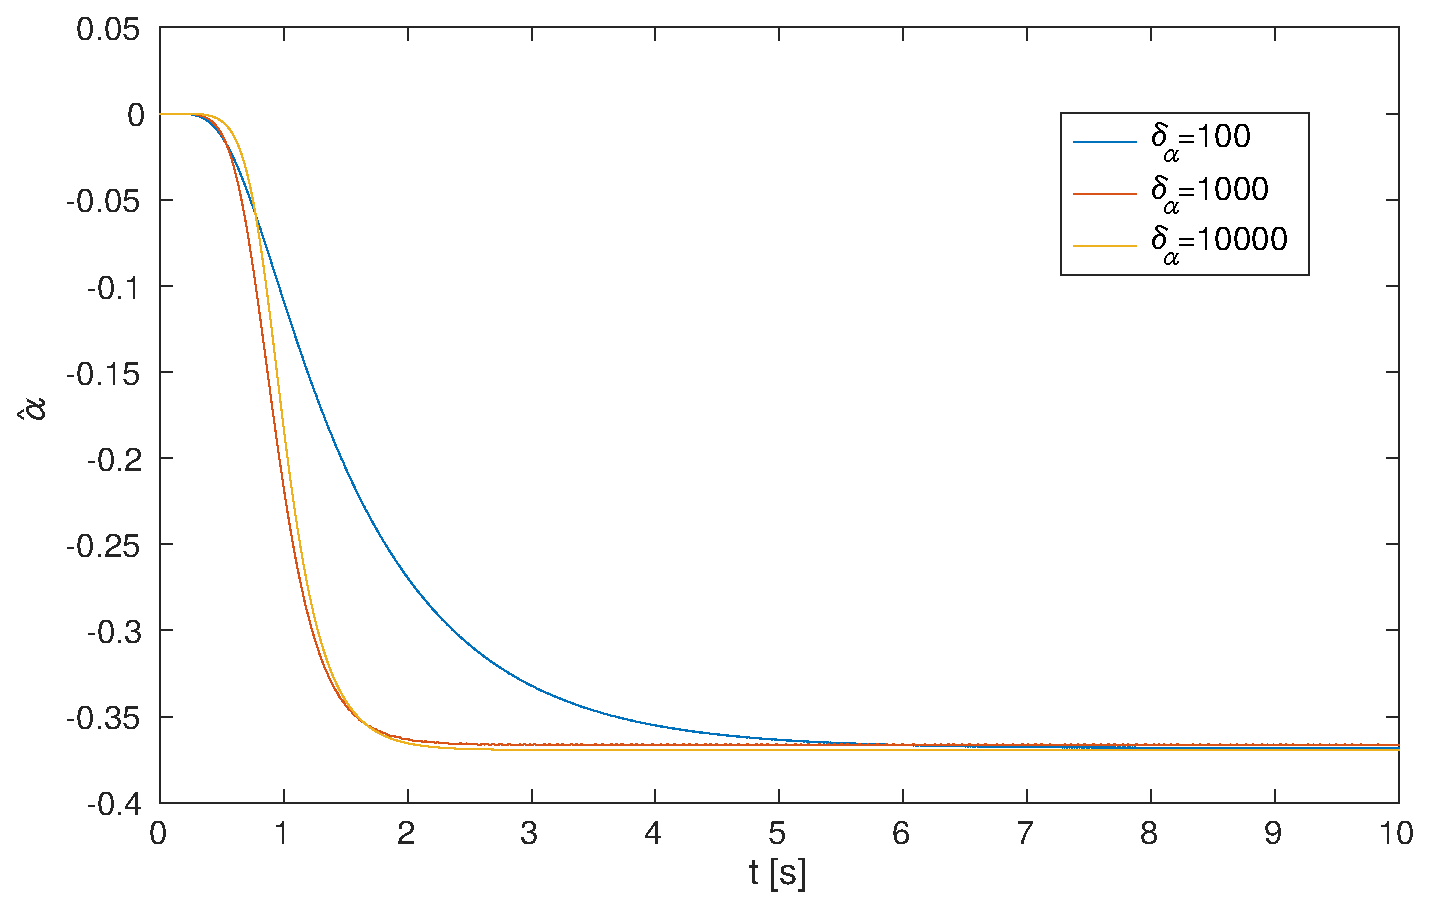
\includegraphics[scale=0.35]{../figure/eps/estimate/1/alpha_hat.eps}}
 \hspace{0.1cm}
 \subfloat[$ \hat{\beta} $の出力]{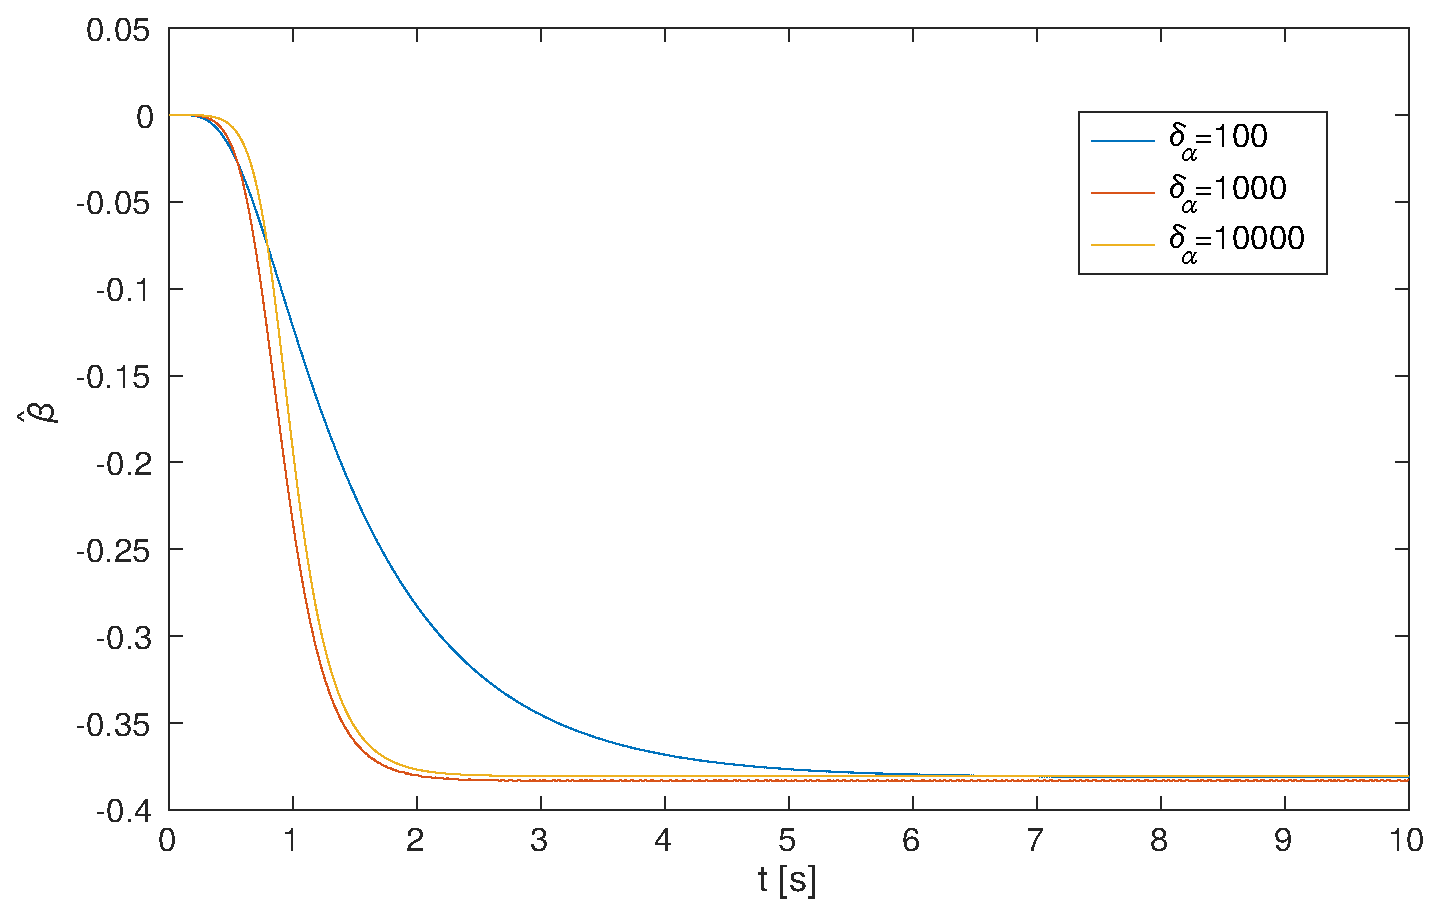
\includegraphics[scale=0.35]{../figure/eps/estimate/1/beta_hat.eps}}
\\
 \vspace{0.5cm}
 \subfloat[$ \hat{\gamma} $の出力]{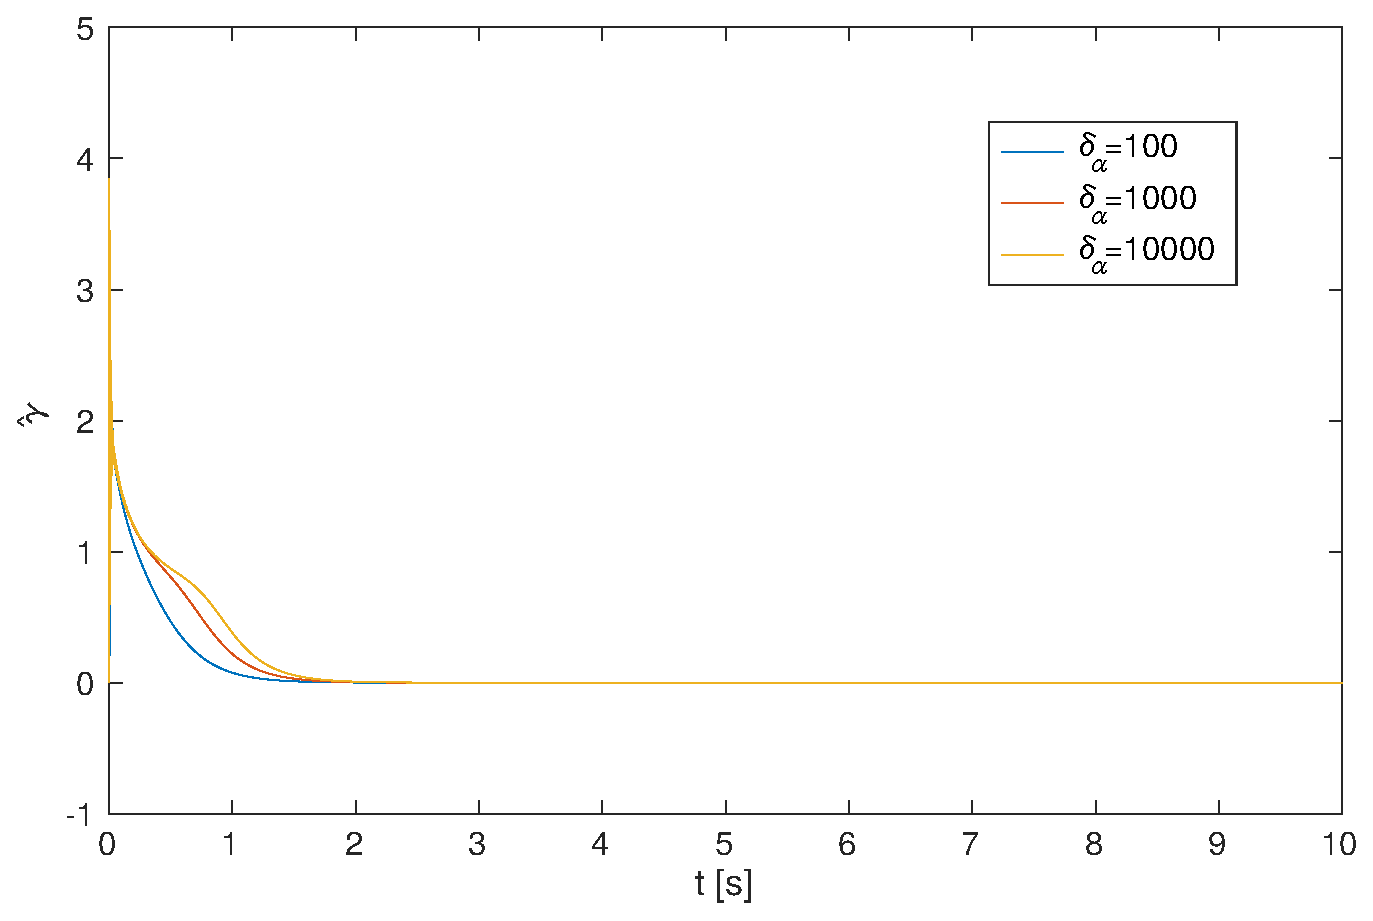
\includegraphics[scale=0.38]{../figure/eps/estimate/1/gamma_hat.eps}}
 \caption{$ r_d = 4 $のときの各推定器の出力$( \delta_{\alpha} = 100, ~ 1000, ~ 10000 )$}
 \label{hatsa1}
\end{figure}
%=================================================
次に,$ r_d = 4 + 0.5{\rm sin}0.5t + {\rm cos}3t -2{\rm sin}5t $のときのシミュレーション結果を{\bf Fig.}{\ref{xa2}}〜{\ref{hatsa2}}に示す.
%=================================================
\begin{figure}[H]
 \begin{center}
  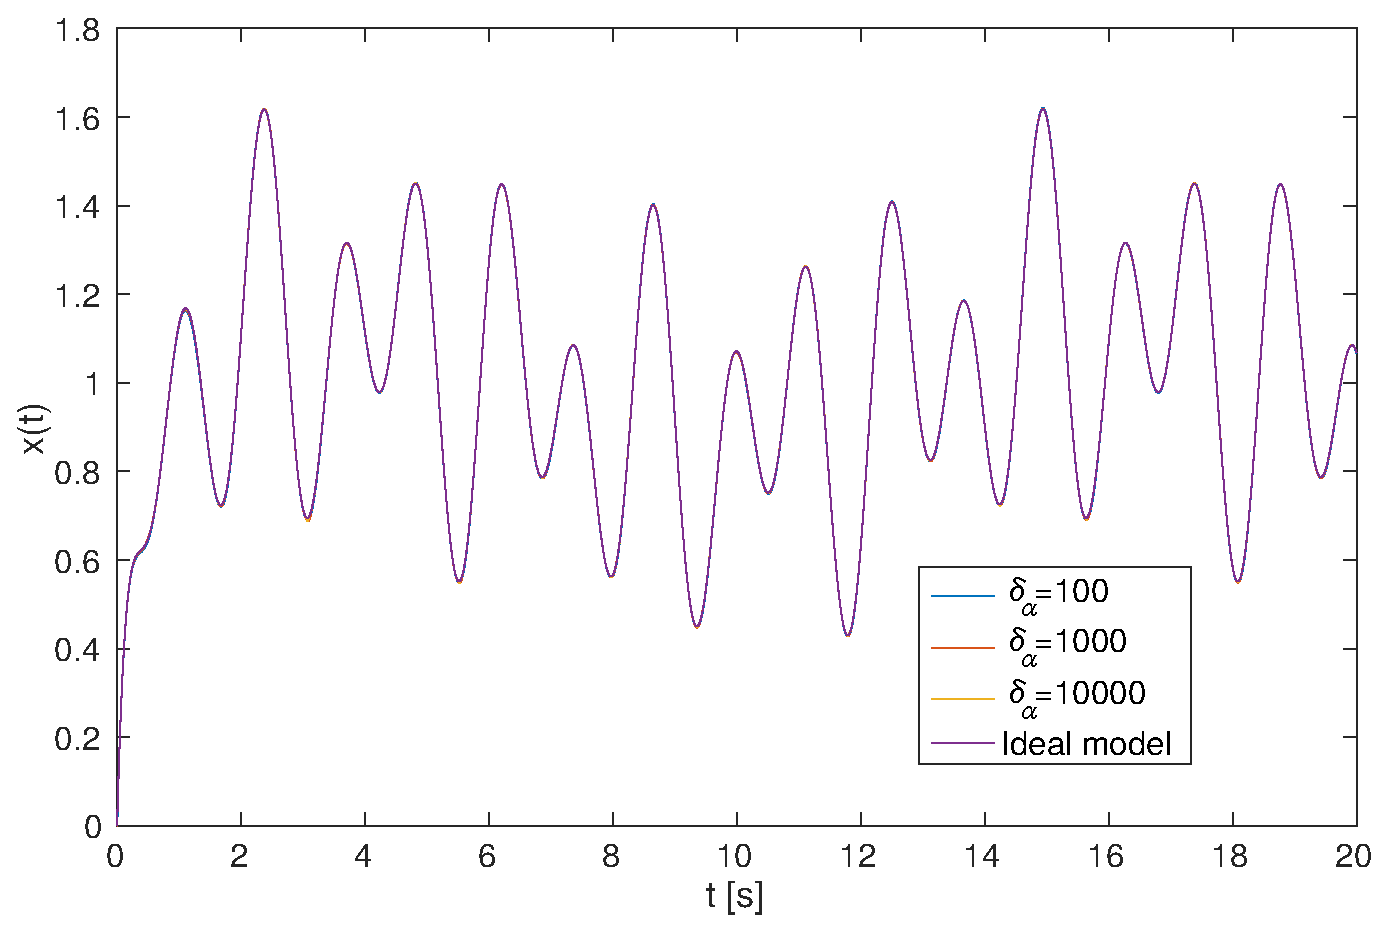
\includegraphics[scale=0.485]{../figure/eps/estimate/2/x.eps}
  \caption{$ r_d = 4 + 0.5{\rm sin}0.5t + {\rm cos}3t -2{\rm sin}5t $のときの理想軌道と$ x(t) $の比較$(\delta_{\alpha} = 100, ~ 1000, ~ 10000 )$}
  \label{xa2}
 \end{center}
\end{figure}
%=================================================
\begin{figure}[H]
 \begin{center}
  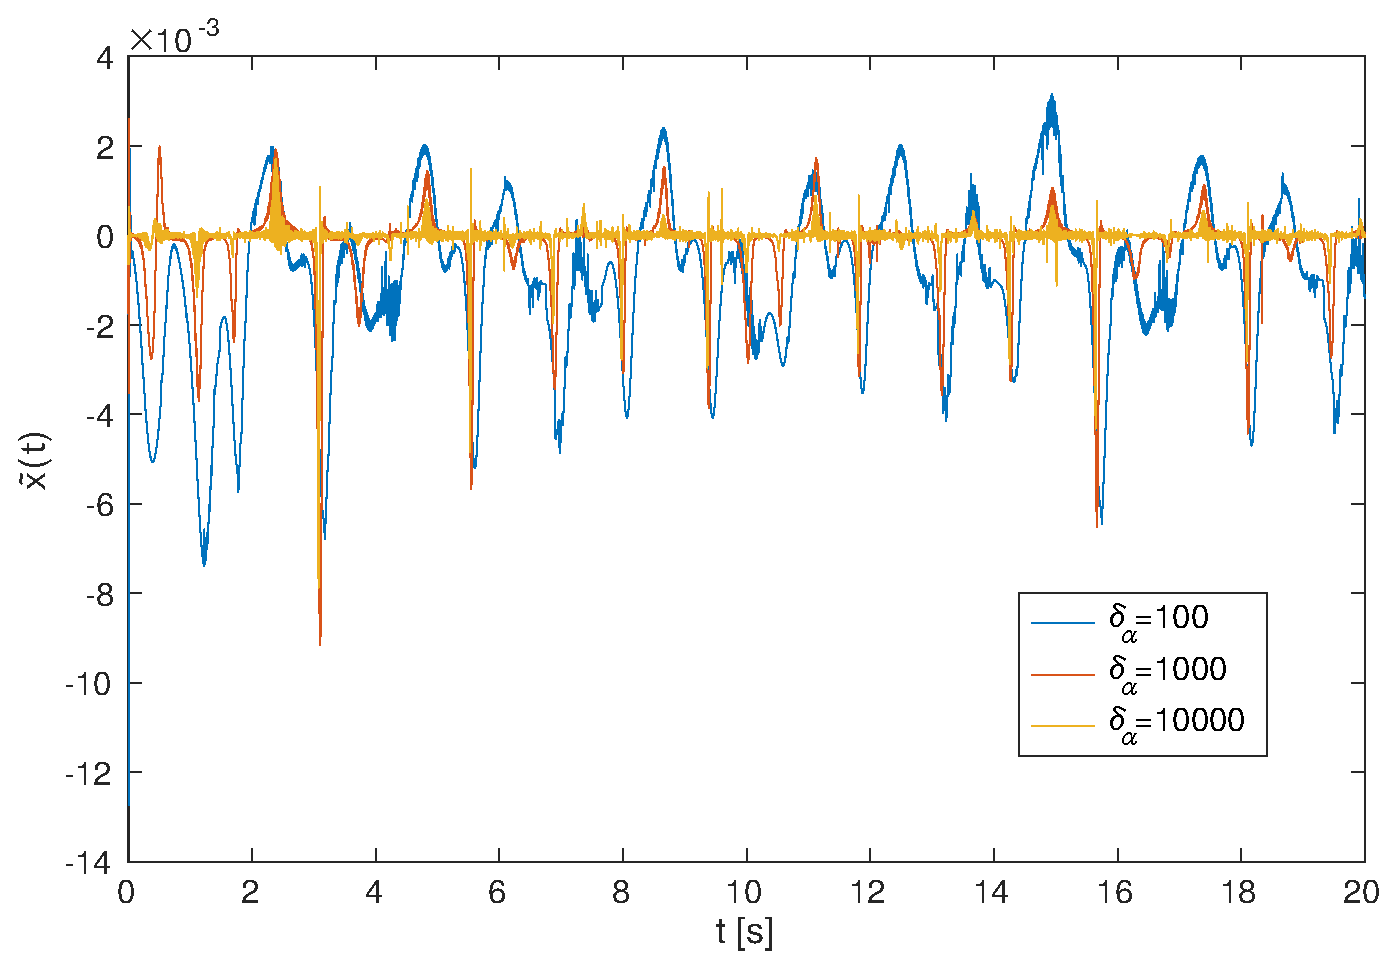
\includegraphics[scale=0.5]{../figure/eps/estimate/2/tilde_x.eps}
  \caption{$ r_d = 4 + 0.5{\rm sin}0.5t + {\rm cos}3t -2{\rm sin}5t $のときの追従誤差$ \tilde{x}(t) $の変化$(\delta_{\alpha} = 100, ~ 1000, ~ 10000 )$}
  \label{tilde_xa2}
 \end{center}
\end{figure}
%=================================================
\begin{figure}[H]
 \begin{center}
  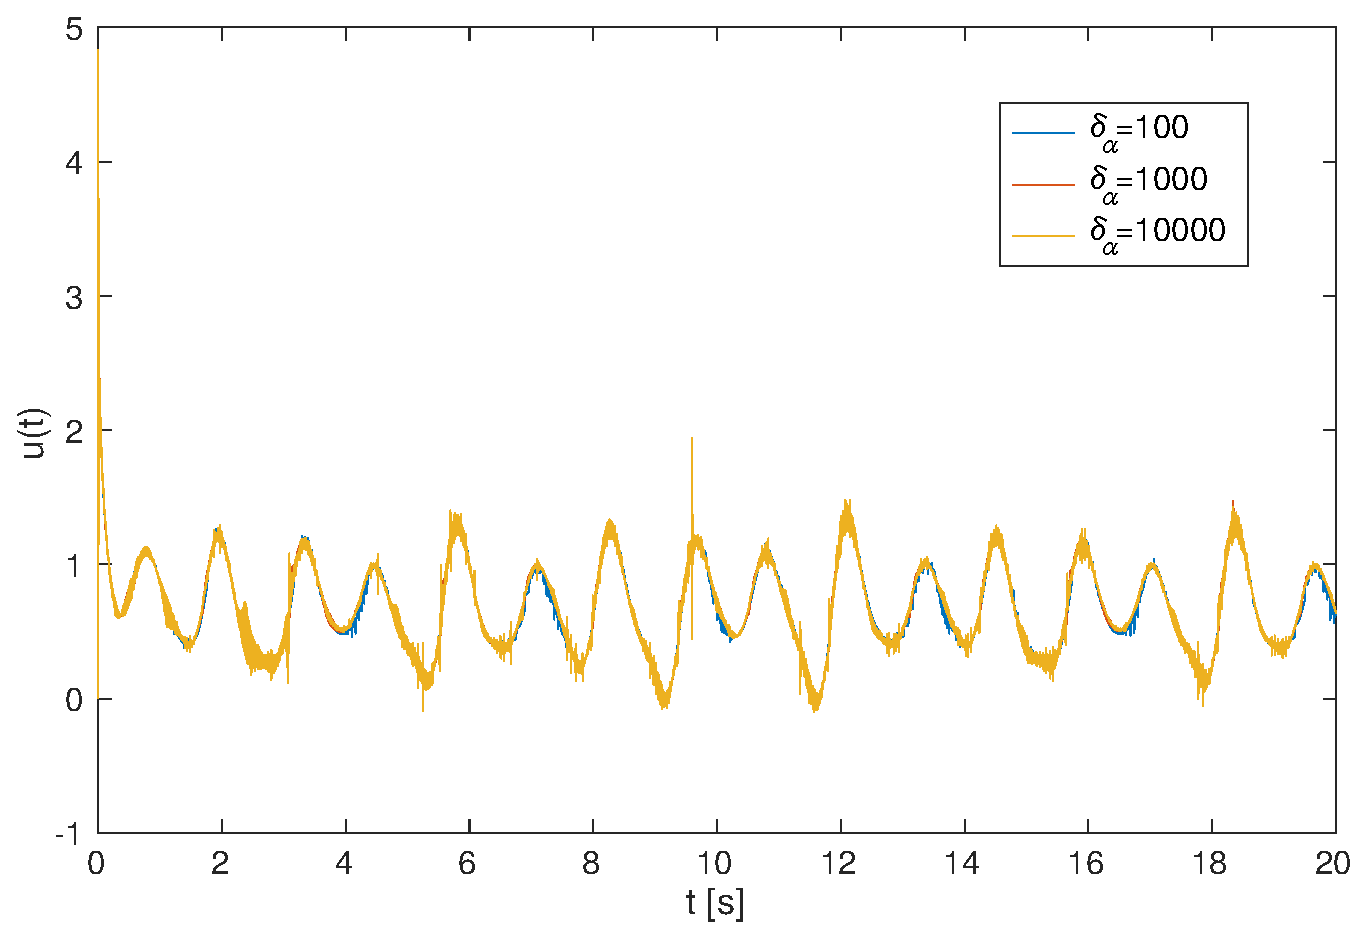
\includegraphics[scale=0.5]{../figure/eps/estimate/2/u.eps}
  \caption{$ r_d = 4 + 0.5{\rm sin}0.5t + {\rm cos}3t -2{\rm sin}5t $のときの入力$ u(t) $の変化$(\delta_{\alpha} = 100, ~ 1000, ~ 10000 )$}
  \label{ua2}
 \end{center}
\end{figure}
%=================================================
\begin{figure}[H]
 \centering
 \subfloat[$ \hat{\alpha} $の出力]{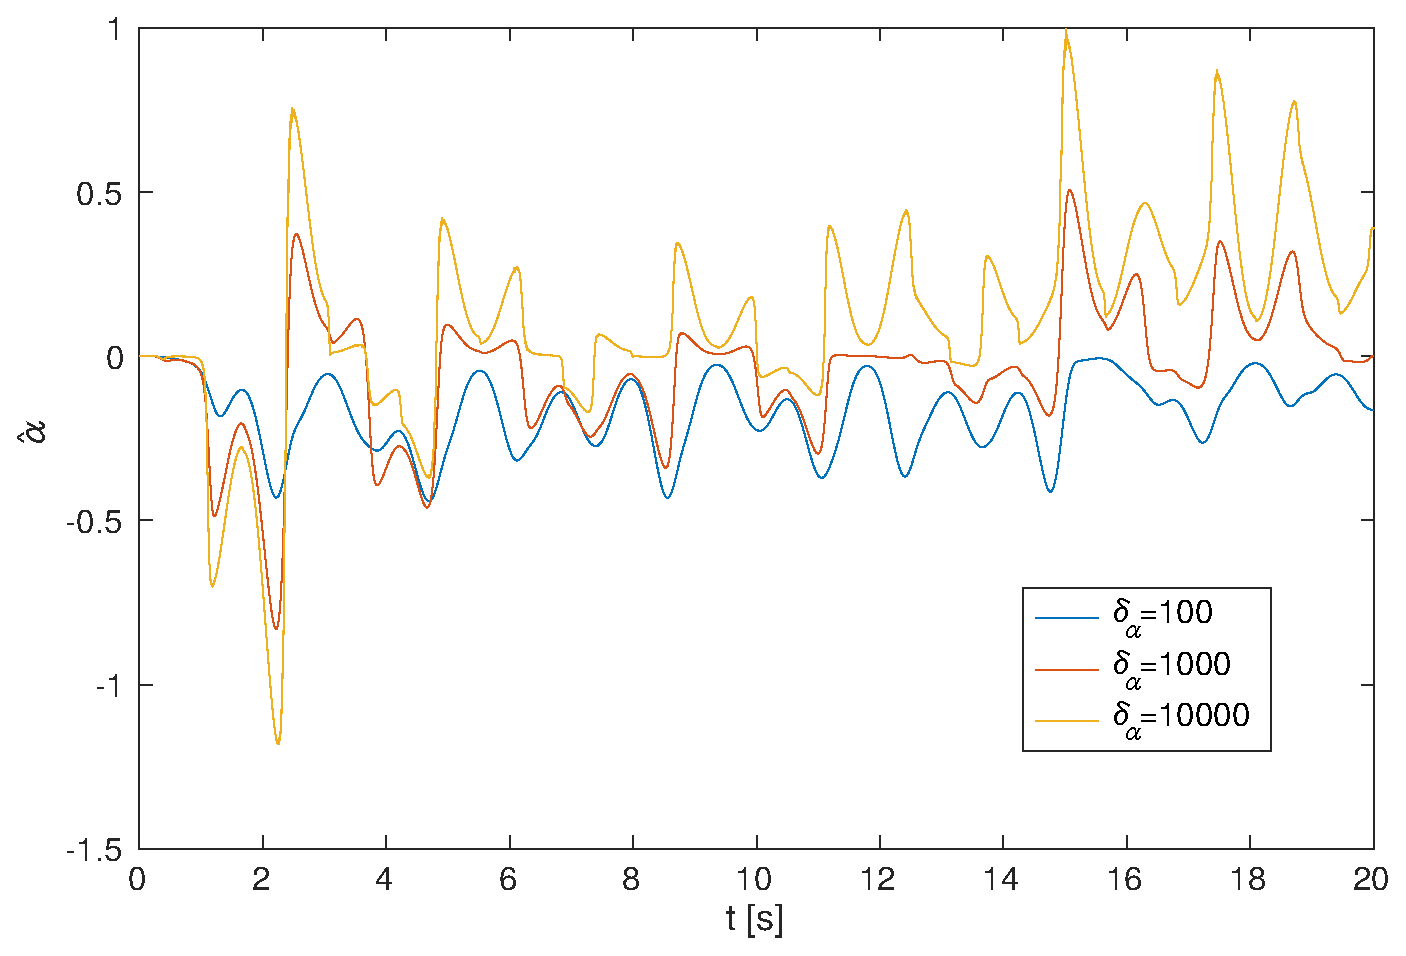
\includegraphics[scale=0.35]{../figure/eps/estimate/2/alpha_hat.eps}}
 \hspace{0.1cm}
 \subfloat[$ \hat{\beta} $の出力]{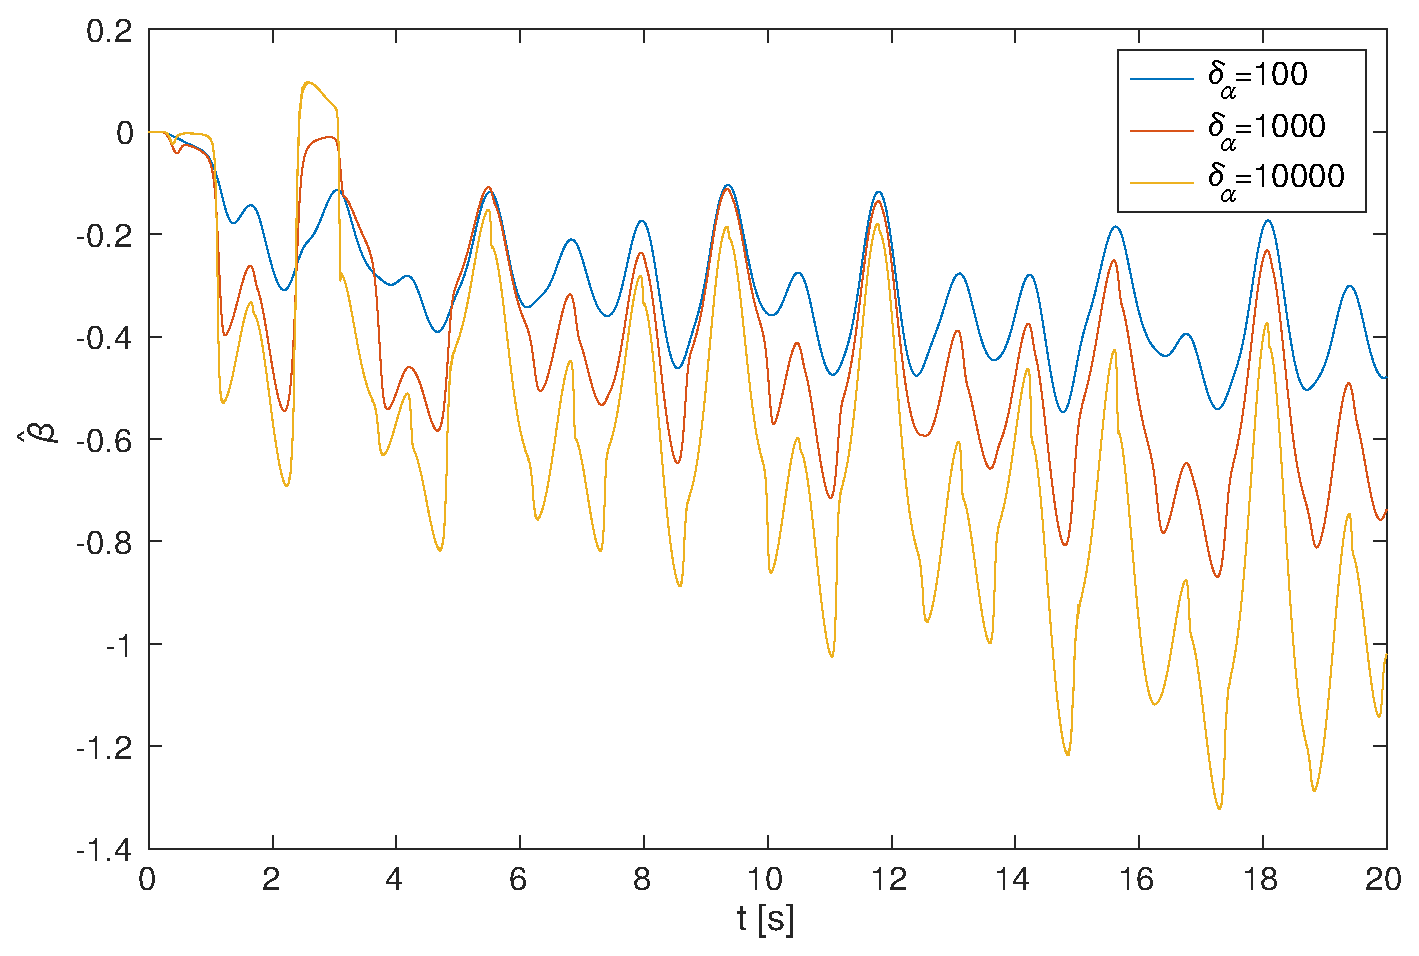
\includegraphics[scale=0.35]{../figure/eps/estimate/2/beta_hat.eps}}
\\
 \vspace{0.5cm}
 \subfloat[$ \hat{\gamma} $の出力]{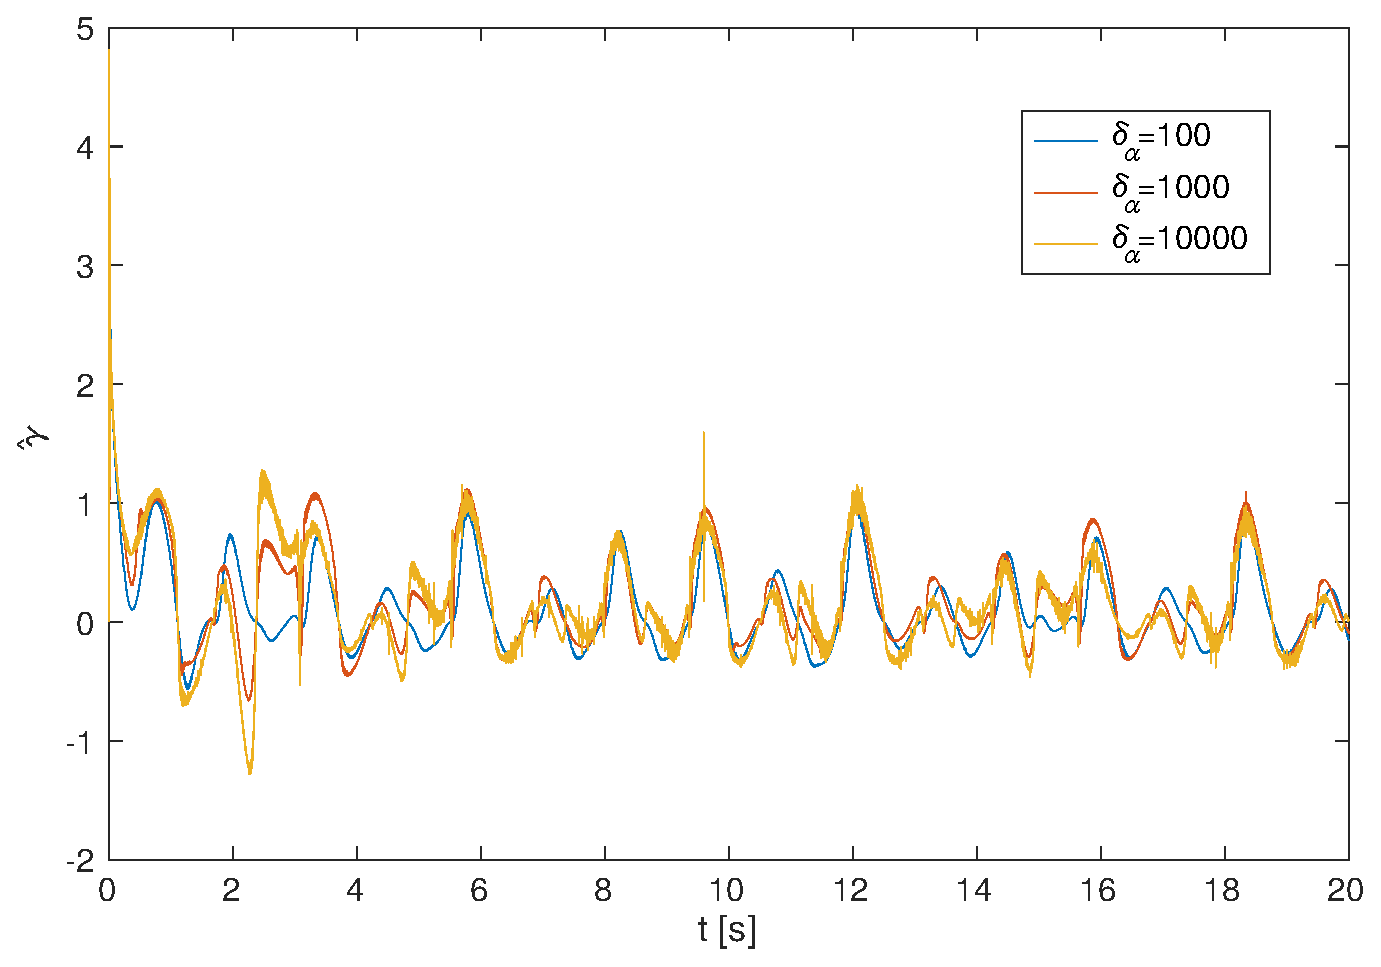
\includegraphics[scale=0.38]{../figure/eps/estimate/2/gamma_hat.eps}}
 \caption{$ r_d = 4 + 0.5{\rm sin}0.5t + {\rm cos}3t -2{\rm sin}5t $のときの各推定器の出力($ \delta_{\alpha} = 100, ~ 1000, ~ 10000 $)}
 \label{hatsa2}
\end{figure}
%=================================================
\section{考察}
%=================================================
まず,$ r_d = 4 $のときについて考察を行う.
{\bf Fig.}{\ref{x1}},{\bf Fig.}{\ref{tilde_x1}}より,入力ゲインのみを変化させたとき,その値が大きいほど理想軌道に近い出力が得られていることが分かる.しかし,追従誤差の値が0に収束していないため,一致はしていない.
また,{\bf Fig.}{\ref{tilde_x1}}と{\bf Fig.}{\ref{tilde_xa1}}から適応ゲインの値の違いによる追従誤差の変化について比較すると,適応ゲインがすべて1の場合では開始から20[s]経過した段階でもある安定な値へと収束しきれていないのに対し,適応ゲインを導入するとある安定な値に収束するのにかかる時間が大幅に改善されていることが分かる.さらに適応ゲインの値が大きいほど,追従誤差が0に近くなっていることが分かる.しかしながら,$ \delta_{\alpha} = 100 $および$ \delta_{\alpha} = 1000 $の場合は,追従誤差が振動しており,安定な値に収束はしていない.

%追従誤差も0に収束してはいない.
次に,$ r_d = 4 + 0.5{\rm sin}0.5t + {\rm cos}3t -2{\rm sin}5t $のときについて考察を行う.
{\bf Fig.}{\ref{x2}}より,入力ゲインのみを変化させたとき,$ \delta = 100 $としたときの出力と理想軌道がおよそ一致していることが分かる.こちらも,ゲインの値が大きいほど,理想軌道に近い出力が得られている.
また,{\bf Fig.}{\ref{tilde_x2}}より追従誤差の値は$ \delta $の値を大きくしてもなお細かく振動しており,収束はしていないことが分かる.さらに,この誤差が0とはなっていないため,出力が完全に一致しているとは言えない.
ここに適応ゲインの変化を加える.
適応ゲインのみを変化させた場合{\bf Fig.}{\ref{xa2}},{\bf Fig.}{\ref{tilde_xa2}}より,
その値が大きいほど理想軌道へ追従していることがわかる.一方,$ r_d =4 $のときとは異なり追従誤差が一定の値に収束する様子は見られず,この変化にノイズのように大きく外れた出力が入っている箇所も見受けられる.
しかしながら,追従誤差の値は適応ゲインを導入する前よりも小さくなっているため,これにより制御性能が改善されたことが分かる.



% {\bf Fig.}{\ref{xa2}}より,$ r_d = 4 + 0.5{\rm sin}0.5t + {\rm cos}3t -2{\rm sin}5t $としたときは,追従誤差の変化にノイズが入っているように見えるが,オーダーが$ 10^{-3} $であるので実際には理想軌道に近い出力が得られている.
% 値が大きいときのほうが全体的な追従誤差は0に近くなっているが,ノイズのように大きく外れている箇所も見られる.
%=================================================
%=================================================
\section{まとめ}
%=================================================
本課題では与えられたシステムに対して追従コントローラを設計しシミュレーションを行なった.これにより,入力ゲインおよび適応ゲインに応じて制御性能が変化することを確認した.
%=================================================
%=================================================
% 参考文献
%=================================================
\begin{thebibliography}{99}
\addcontentsline{toc}{section}{参考文献}
\bibitem{1} 大屋勝敬,”車両制御特論 Advanced Vehicle Control ”,九州工業大学 機械知能工学研究系,pp.37,2011.
\bibitem{2} 大屋勝敬,”車両制御特論 MATLAB+Simulink の利用法 ”,九州工業大学 機械知能工学研究系,2013.
\end{thebibliography}
%=================================================
\end{document}
